% Cleiber Marques da Silva -- cleiber.dev@gmail.com
% Filipe Medeiros de Almeida -- f.almeida87l@gmail.com
% 2009-01
% ----------------------------------------------------------------------- %
% Mobilidade em Redes IP: An�lise dos Protocolos MIPv6 e HMIPv6
%
% Arquivo: monografia.tex (principal)
% ----------------------------------------------------------------------- %

\documentclass[ruledheader]{abnt}

\usepackage{estilo-monografia}

\usepackage{url,subfigure,graphicx}
\usepackage{listings,color}

\definecolor{colBack}{rgb}{1,1,.98}
\definecolor{colKeys}{rgb}{0,0,0}
\definecolor{colIdentifier}{rgb}{0,0,0.9}
\definecolor{colComments}{rgb}{.4,.4,.4}
\definecolor{colString}{rgb}{0,0,0.6}

\lstset{language=C,basicstyle=\ttfamily\footnotesize,tabsize=3,frame=single,showtabs=false,showspaces=false,numbers=left,numberstyle=\tiny,linewidth=0.98\linewidth,xleftmargin=21pt,tab=$\to$,float=tbph,extendedchars,breaklines,showstringspaces=false,identifierstyle=\color{colIdentifier},keywordstyle=\color{colKeys},stringstyle=\color{colString},commentstyle=\color{colComments},backgroundcolor=\color{colBack},columns=flexible,captionpos=b,aboveskip=\bigskipamount}


\usepackage{makeglo}
\makeglossary

\begin{document}

% inclus�o das partes iniciais do documento
% ----------------------------------------------------------------------- %
% Onde ser�o inseridas informa��es que ir�o aparecer na capa e na
% folha de rosto
%
% Arquivo: capa.tex
% ----------------------------------------------------------------------- %


\titulo{Plataforma para o Estudo de Mobilidade na Camada de Rede}

\autor{Cleiber Marques da Silva\\ Filipe Medeiros de Almeida}

\orientador{Prof. Eraldo Silveira e Silva}
% ou \orientador[Orientadora:\\]{Prof. Dra. Nome da orientadora}

%\coorientador{Nome do co-orientador}
% ou \coorientador[Co-orientadora:\\]{Prof. Dra. Nome da orientadora}

\comentario{Monografia apresentada � Coordena��o do Curso Superior de Tecnologia
em Sistemas de Telecomunica��es do Instituto Federal de Educa��o, Ci�ncia e
Tecnologia de Santa Catarina para a obten��o do diploma de Tecn�logo em Sistemas
de Telecomunica��es.}


\instituicao{Curso Superior de Tecnologia em Sistemas de Telecomunica��es \par 
	Instituto Federal de Educa��o, Ci�ncia e Tecnologia de Santa Catarina}

\local{S�o Jos� -- SC}

\data{Mar�o / 2009}

\capa

\folhaderosto

% ----------------------------------------------------------------------- %
% Onde ser�o inseridas informa��es que ir�o compor a folha de aprova��o
%
% Arquivo: folhadeaprovacao.tex
% ----------------------------------------------------------------------- %

\begin{folhadeaprovacao}
Monografia sob o t�tulo \textit{``Mobilidade em Redes IP: An�lise dos Protocolos MIPv6 e HMIPv6''}, defendida por Cleiber Marques da Silva e Filipe Medeiros de Almeida e aprovada em 06 de Mar�o de 2009, em S�o Jos�, Santa Catarina, pela banca examinadora assim constitu�da:

\setlength{\ABNTsignthickness}{0.4pt}
\setlength{\ABNTsignwidth}{10cm}
\setlength{\ABNTsignskip}{3.5cm}

\assinatura{Prof. Dr. Eraldo Silveira e Silva \\ Orientador}
\assinatura{Prof. Dr. Nome de Um Membro da Banca \\ CEFET / SC}
\assinatura{Prof. Dr. Nome de Outro Membro da Banca \\ Departamento de Automa��o e Sistemas - UFSC}

\end{folhadeaprovacao}

% ----------------------------------------------------------------------- %
% Pequena dedicat�ria ou uma ep�grafe (uma cita��o pertinente ao seu
% trabalho ou que represente o seu modo de pensar.)
% 
%
% Arquivo: dedicatoria.tex
% ----------------------------------------------------------------------- %

\vspace*{\fill}

{ \raggedleft


\textit{In a world without fences and walls \\
who needs Windows and Gates.}


}
% ----------------------------------------------------------------------- %
% Um pequeno texto para agradecer �queles que contribu�ram de maneira
% relevante � elabora��o do trabalho 
%
% Arquivo: agradecimentos.tex
% ----------------------------------------------------------------------- %

\chapter*{Agradecimentos}

Aos meus queridos pais e familiares, que nunca mediram esfor�os para que eu
pudesse atingir meus objetivos. Al�m do apoio, confian�a, dedica��o e presen�a
constante em todos os momentos da minha vida.

Aos meus amigos que ao longo dos �ltimos anos, trabalhei, aprendi, festejei,
troquei ideias. A estes quero agradecer de forma especial pelo incentivo,
apoio e amizade.

Ao professor Eraldo, pelos esclarecimentos das d�vidas, todos os coment�rios
sempre �teis, colobora��o e dedica��o. Al�m da prontid�o para me auxiliar em
todos os momentos durante a elabora��o deste trabalho.

\textbf{\textit{Cleiber Marques da Silva}}


\vspace{2cm}

Aos meus pais e familiares, pela base s�lida que sempre me deu for�a para 
encarar a vida de frente. Principalmente aos meus pais, por serem um exemplo de
for�a de vontade, mas, que acima de tudo, me ensinaram a percorrer meu pr�prio 
caminho.

Aos amigos com quem tive todo o prazer em trocar experi�ncias, tanto em quest�es
academicas quanto no amadurecimento como pessoa, sendo na nossa querida 
institui��o de tijolos � vista, nas nossas festas ou nos bares da regi�o.

A todos os professores que contribu�ram decisivamente para a minha, e nossa,
forma��o academica, profissional e pessoal. Em especial ao meu orientador 
professor Eraldo, por todo o conhecimento passado, pelas excelentes supervis�es,
orienta��o e por sempre acreditar no potencial dos alunos.

\textbf{\textit{Filipe Medeiros de Almeida}}

% ----------------------------------------------------------------------- %
% Pequeno texto que em poucas palavras consegue expressar o trabalho.
% O resumo deve ser concebido de forma tal que, uma pessoa ao ler o resumo
% possa entender sobre qual assunto este trabalho trata.
%
% Arquivo: resumo.tex
% ----------------------------------------------------------------------- %

\begin{resumo}
A investiga��o de tecnologias que possibilitam a mobilidade de terminais no
�mbito da Internet vem ganhando um grande espa�o na comunidade cient�fica. As
solu��es de mobilidade na camada de rede, tal como o IP M�vel e seus derivados,
apresentam-se como uma forma transparente e elegante de tratar o deslocamento de
um n� m�vel entre sub-redes. Neste trabalho descreve-se a implementa��o de uma
plataforma de testes baseada em m�quinas virtuais UML com fins facilitar os
estudos dos referidos protocolos, e a implementa��o de uma vers�o experimental
do IP M�vel Hier�rquico. Tamb�m s�o apresentados resultados sobre a efici�ncia e
funcionamento dos protocolos estudados, a partir de cen�rios de testes
realizados sobre a plataforma.

\textbf{Palavras-chave:} IP M�vel, IP M�vel Hier�rquico, IP M�vel para o Linux,
Linux Modo Usu�rio, Plataforma de Testes.
\end{resumo}

% ----------------------------------------------------------------------- %
% Tradu��o do resumo para a l�ngua inglesa.
% 
% 
%
% Arquivo: abstract.tex
% ----------------------------------------------------------------------- %

\begin{abstract}
The investigation of technologies that enable the mobility of terminals in
the Internet has gained a large space in the scientific community. The
solutions for mobility in the network layer, such as Mobile IPv6 and its
derivatives, appear as a transparent and elegant way to deal with the
displacement of a mobile node between subnets. This work describes the
implementation of a testing platform based on UML virtual machines with the
purpose of facilitating studies of these protocols, specifically the Mobile IPv6
and the Hierarchical Mobile IPv6. The lack of an updated code for the 
last one motivated an implementation of a experimental version of
the Hierarchical Mobile IP. As an additional contribution, it is discussed 
preliminary results on the operation and performance of the studied protocols,
extracted from test scenarios performed on the platform.

\textbf{Keywords:} Mobile IP, Mobile IP Hierarchical, Mobile IP for Linux,
User Mode Linux, Platform of tests.
\end{abstract}


% listas autom�ticas: sum�rio, lista de figuras e lista de tabelas
\tableofcontents
\listoffigures
\listoftables

% ----------------------------------------------------------------------- %
% Onde ser� incluido o gloss�rio
%
% Arquivo: glossario.tex
% ----------------------------------------------------------------------- %
\renewcommand{\glossaryname}{Gloss�rio}

\Glossary{N� m�vel}{� o terminal de rede que pode trocar seu ponto de acesso a internet sem deixar de ser alcan��vel via seu endere�o domiciliar}

\Glossary{Endere�o domiciliar}{� o endere�o est�tico associado ao n� m�vel na rede domiciliar}

\Glossary{\textit{Link} domiciliar}{\textit{link} onde o prefixo de subrede do n� m�vel � definido}

\Glossary{\textit{Link} externo}{algum \textit{link} que n�o seja \textit{link} domiciliar do n� m�vel}

\Glossary{\textit{Care-of-address}}{endere�o IP dado ao n� m�vel quando estiver em um \textit{link} externo, o prefixo da rede deste endere�o � o da rede externa}

\Glossary{N� correspondente}{� o n� com quem o n� m�vel esta se correspondendo, pode ser m�vel ou fixo}

\Glossary{Agente domiciliar}{� um roteador no \textit{link} domiciliar com quem o n� m�vel registra seu \textit{care-of-address} sempre que esta em um \textit{link} externo}

\Glossary{Movimento}{� uma troca de ponto de acesso na Internet}

\Glossary{\textit{Binding}}{� associa��o do endere�o domiciliar do n� m�vel com seu \textit{care-of-address}}

\Glossary{Roteador de acesso}{� o roteador padr�o do n� m�vel, recebe os dados de sa�da do n� m�vel}

\Glossary{\textit{Mobility Anchor Point}}{� um roteador localizado na rede visitada, o MAP � usado como um agente domiciliar pelo n� m�vel. Um ou mais MAPs podem existir em uma rede visitada}

\Glossary{N� m�vel HMIPv6}{� um n� m�vel capaz de receber e processar mensagens do roteador padr�o que contenham a op��o MAP. Um n� m�vel HMIPv6 deve ser apto para enviar \textit{Binding Updates} locais com o bit M ligado}

\Glossary{Regional \textit{care-of-address}}{� o endere�o obtido pelo n� m�vel na rede visitado com o mesmo prefixo de rede do MAP. Ele � auto-configurado quando recebe a op��o de MAP divulgada nas mensagens do roteador padr�o}

\Glossary{\textit{Link care-of-address}}{� o endere�o configurado pelo n� m�vel com o mesmo prefixo do roteador padr�o. Uma simples refer�ncia ao care-of-address}

\Glossary{\textit{Binding Update} local}{� o \textit{Binding Update} que o n� m�vel envia para o MAP fazer a associa��o do LCoA com o RCoA}
\clearpage
\printglossary

% inclus�o dos cap�tulos
% ----------------------------------------------------------------------- %
% Arquivo: introducao.tex
% ----------------------------------------------------------------------- %

\chapter{Introdu��o}
\label{c_introducao}

\section{Motiva��o}
\label{ci_s_motivacao}

A utiliza��o de dispositivos m�veis para o acesso a Internet vem crescendo
acentuadamente nos �ltimos anos. As novas aplica��es multim�dias incentivam esta
expans�o, aliadas a uma variedade de novas tecnologias de acesso sem fio que
permitem suportar taxas de transmiss�o em n�veis relativamente altos. Algumas
destas tecnologias, consideradas como camada de enlace e f�sica do
ponto de vista da arquitetura TCP-IP, possuem mecanismos para o tratamento de
movimentos entre esta��es base, minimizando os efeitos destas opera��es para o
usu�rio.

Contudo, a utiliza��o de redes IP em situa��es de mobilidade pode impactar
consideravelmente as camadas superiores, independentemente da tecnologia de
acesso. Comunica��es em andamento podem ser interrompidas de forma brusca e
novas comunica��es podem ser inviabilizadas quando um terminal m�vel se
movimenta para uma nova subrede IP. Este fato adv�m do car�ter de
posicionamento topol�gico dos endere�amentos IP. Uma mudan�a de subrede
inviabiliza, a priori, a utiliza��o de um endere�o IP da rede de origem, dado
que os protocolos de roteamento subjacentes n�o podem atualizar as rotas em
tempo real, evidenciando um problema de escalabilidade.

Uma s�rie de propostas da IETF vem de encontro a este problema. Estas propostas
orbitam em torno do protocolo IP m�vel, nas vers�es 4 e 6. O estudo e teste
destes protocolos envolve, normalmente, arranjos relativamente complexos com
estruturas de rede sem fio al�m de entidades associadas aos protocolos de
mobilidade da camada de rede. Esta constata��o � um dos fatores primeiros que
motivaram o desenvolvimento deste trabalho.


\section{Objetivos}

O presente trabalho visa o desenvolvimento de uma plataforma para o estudo
de protocolos de mobilidade na camada de rede, em particular os protocolos
MIPv6 e HMIPv6.

Como especifica��es b�sicas desta plataforma pode-se enumerar:
\begin{itemize}
 \item a execu��o real dos protocolos, de forma que se possa configur�-los e
execut�-los de forma muito pr�xima de cen�rios reais;
\item facilidades de constru��o de cen�rios sem a necessidade de arranjos de
rede sem fio, reproduzindo, no entanto, os movimentos que impactam a camada de
rede;
\item pronta disponibilidade de ferramentas de medi��o, an�lise de tr�fego, bem
como protocolos de roteamento din�micos;
\end{itemize}


\section{Organiza��o do texto}
\label{ci_s_organizacao}

Este trabalho est� organizado da seguinte forma. O cap�tulo 2 resume os dois
protocolos de mobilidade de interesse: o protocolo IP m�vel vers�o 6, MIPv6 e
sua extens�o, o protocolo IP m�vel hier�rquico, HMIPv6. O cap�tulo 3 apresenta
a plataforma de mobilidade desenvolvida com apoio de m�quinas virtuais. Tendo
em vista que foram realizadas modifica��es em um c�digo aberto do MIPv6, para
que se comportasse tal como o HMIPv6, no cap�tulo 4 � apresentada uma vis�o
geral deste c�digo, bem como as modifica��es realizadas no mesmo para a
obten��o do HMIPv6. No cap�tulo 5 a plataforma de mobilidade � explorada para a
constru��o de alguns cen�rios de mobilidade com o MIPv6 e o HMIPv6. O cap�tulo
6 conclui e apresenta as perspectivas futuras de trabalhos usando a plataforma.
% ----------------------------------------------------------------------- %
% Arquivo: mipv6.tex
% ----------------------------------------------------------------------- %
\chapter{Protocolos de Mobilidade da camada Rede}

\section{O Problema da Mobilidade na Camada de Rede}
\label{s_mipv6}

Em redes IP, cada pacote integrante de um fluxo de pacotes entre dois pontos
comunicantes, � encaminhado em fun��o do seu endere�o de IP destino. Cabe ao
protocolo de camada de rede, chamado \acf{IP} \cite{rfc791}, determinar rotas e
encaminhar pacotes para que eles alcancem o seu destino. Em muitos casos, quando
as redes s�o complexas, os protocolos de roteamento proporcionam a descoberta da
localiza��o dos destinos dinamicamente. Alguns exemplos de protocolos de
roteamento s�o o \ac{OSPF}, o \ac{RIP} e o \ac{BGP}.

Os endere�os IP acabam definindo a localiza��o geogr�fica de um hospedeiro. Os
protocolos atuais da \textit{Internet} assumem que o n� n�o muda seu endere�o IP
durante uma comunica��o, ou seja, n�o altera o seu ponto de conex�o � rede.

Caso um n� mude seu ponto de conex�o, ele dever�, normalmente, configurar um
novo endere�o IP e, possivelmente, um novo roteador padr�o. Se uma comunica��o
estiver estabelecida quando o n� efetuar a mobilidade, os protocolos de
roteamento n�o corrijir�o a rota para o novo destino. Para continuar a
comunica��o, sua nova rota deveria ser propagada para toda estrutura de
roteamento da rede. Obviamente esta alternativa � inaceit�vel, pois seria
invi�vel fazer isso em uma rede IP, por quest�es de escalabilidade.

Com a inten��o de permitir que os n�s possam se movimentar para diferentes
subredes e continuar suas comunica��es, a IETF prop�s o \acf{MIP} que garante
que os pacotes sejam roteados para os n�s m�veis. Existem duas varia��es para o
MIP: uma para o \ac{IPv4} \cite{rfc3344} e outra para o \ac{IPv6}
\cite{rfc3775}. O foco deste trabalho ser� na vers�o para o IPv6, pois este
possui algumas vantagens sobre o IPv4 como maior n�mero de endere�os, suporte
nativo para seguran�a, possibilidade de autoconfigura��o e suporte ao MIP.

Em adi��o, a IETF prop�s o HMIPv6 \cite{rfc4140} que permite aumentar o
desempenho do protocolo MIPv6 atrav�s do tratamento localizado da mobilidade um
mesmo dom�nio. Na sequ�ncia, ser�o apresentados brevemente os referidos
protocolos.

\section{Vis�o Geral do Funcionamento do MIPv6}
\label{sub_mipv6_func}

O protocolo IPv6 m�vel (MIPv6) tem por objetivo, portanto, permitir que n�s IPv6
se desloquem, de forma transparente, entre subredes, com diferentes
tecnologias de acesso, tais como \textit{Ethernet} e \textit{Wireless LAN}, e
mantenham as comunica��es em andamento. Novas comunica��es tamb�m ser�o
possibilitadas. Sem suporte ao MIPv6 todos os pacotes destinados ao n� m�vel,
quando ele estiver fora de sua rede origem, seriam perdidos.

No contexto do MIPv6 um n� m�vel est� sempre acess�vel por um mesmo endere�o IP,
independente de seu ponto de conex�o com a \textit{Internet}. Este endere�o �
chamado de endere�o domiciliar e � o endere�o IPv6 fixo global do n� m�vel na
sua rede de origem. Todos os n�s correspondentes utilizam este endere�o para se
comunicar com o n� m�vel.

Quando um n� m�vel estiver fora de sua rede de origem ele ter� no m�nimo
dois endere�os atribu�dos a sua interface de rede:
\begin{enumerate}
\item Um endere�o domiciliar que ser� permanente, e que, supostamente ser�
utilizado pelos n�s correspondentes em suas sess�es de comunica��o;
\item Um endere�o chamado de \ac{CoA}, que se refere a
rede visitada. A cada nova rede ser� configurado um CoA.
\end{enumerate}

O CoA pode ser obtido pelas formas convencionais do IPv6, ou seja, por
\textit{stateless autoconfiguration} \cite{rfc2462}, no qual o endere�o � gerado
por meio de informa��es divulgadas pelos roteadores das subredes, ou por 
\textit{stateful autoconfiguration}, onde o endere�o e outros par�metros de
configura��o s�o providos diretamente de um servidor, por exemplo, os mecanismos
\ac{DHCPv6} e \ac{PPPv6}.

Na rede visitada, ap�s detectar o movimento e configurar seu CoA, o n� m�vel
envia uma mensagem \ac{ICMPv6} de \ac{BU} para seu Agente Domiciliar, para que
este fa�a a associa��o de seu endere�o domiciliar com o seu CoA. Esta informa��o
� registrada em um \textit{cache} local do Agente Domiciliar. Este, em resposta,
envia um \ac{BA} para o n� m�vel. O Agente Domiciliar passa, ent�o, a atuar como
um \textit{proxy}, interceptando todos os pacotes com destino ao n� m�vel e
enviando-os, via t�nel, para este n�. Opcionalmente, o n� m�vel pode tamb�m
informar ao n� correspondente sua localiza��o. Neste caso, assim que o n�
correspondente atualizar seu \textit{cache}, ele encaminhar� os pacotes
diretamente ao n� m�vel.

Duas formas de comunica��o podem ser realizadas entre o n� m�vel e o
correspondente (ver figura \ref{f_mipv6}). No primeiro modo, com tunelamento
bidirecional, todos os pacotes s�o encaminhados via Agente Domiciliar e o o n�
correspondente n�o precisa ter suporte ao MIPv6. Os pacotes com origem no n�
correspondente s�o roteados para o Agente Domiciliar e este envia ao n� m�vel
via t�nel. No sentido contr�rio, pacotes enviados pelo n� m�vel, com destino ao
n� correspondente, s�o enviandos, via t�nel, ao Agente Domiciliar (t�nel
reverso) e estes s�o roteados normalmente da rede domiciliar para o n�
correspondente. O Agente Domiciliar utiliza \textit{proxy Neighbor Discovery}
para interceptar os pacotes com destino ao n� m�vel.

O segundo modo, mais eficiente, � chamado de \textit{``otimiza��o
de roteamento''}. O n� m�vel, adicionalmente ao registro com o Agente
Domiciliar, tamb�m faz uma associa��o do seu CoA com o n�
correspondente e este pode come�ar a endere�ar os pacotes diretamente ao
CoA, melhorando a escabilidade do protocolo e minimizando o
tr�fego de rede.

\begin{figure}[!htpb]
	\centering
	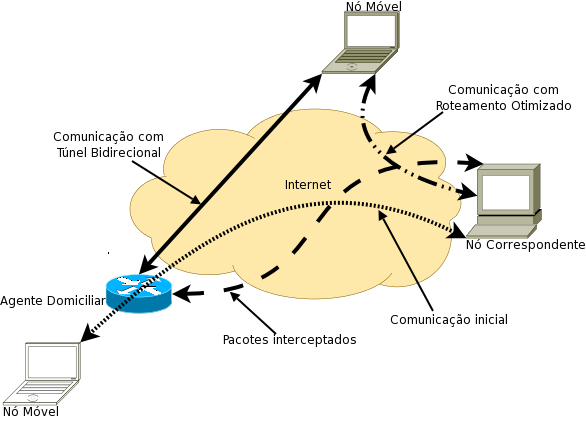
\includegraphics[scale=.5]{figs/mipv6}
	\caption{Modos de opera��o simplificados do MIPv6}
	\label{f_mipv6}
\end{figure}

Como citado anteriormente, enquanto estiver em uma rede visitada, o n� m�vel
ter� mais de um endere�o configurado em sua interface: o endere�o domiciliar e
um ou mais CoA. Ele poder� usar qualquer um destes como
endere�o fonte para se comunicar. Com o intuito de manter a traspar�ncia para
as camadas superiores � de rede, o n� m�vel ir� utilizar geralmente seu endere�o
domiciliar. � interessante observar que os pacotes enviados pelo n� m�vel
dever�o ser modificados, inserindo-se o CoA no campo
endere�o de origem e, movendo o endere�o domiciliar para o cabe�alho 
de mobilidade \textit{home address}. No receptor do pacote, estas altera��es
devem ser revertidas para manter a transpar�ncia para as camadas superiores.

\subsection{O Procedimento de Handover no MIPv6}
\label{sub_mipv6_handover}

Conforme a \ac{RFC} 3775 \cite{rfc3775}, o \textit{Handover} de camada 3 pode
ser definido como o processo em que o n� m�vel muda seu ponto de acesso, percebe
a mudan�a de subrede, configura um novo CoA e o registra
com o seu Agente Domiciliar/correspondentes. Note que o
gerenciamento do \textit{handover} pode se dar em diferentes camadas da
arquitetura de rede. O \textit{handover} de camada enlace refere-se, por
exemplo, a descoberta e conex�o h� um novo ponto de acesso sem necessariamente
causar um \textit{handover} de camada 3. J� o \textit{handover} na camada rede,
no caso da arquitetura IPv6, envolve:
\begin{enumerate}
 \item Descoberta de um novo roteador;
 \item Auto configura��o do CoA;
 \item Teste de duplicidade do CoA (DAD), e;
 \item Registro com o agente domiciliar e o n� correspondente.
\end{enumerate}

O in�cio de um \textit{handover} de camada 3 se d� a partir do protocolo
\ac{ND} presente no IPv6. Este protocolo utiliza-se, dentre
outros, dos mecanismos \ac{RD}  para realizar a detec��o de
uma nova rede.

O RD \cite{rfc2461} � o mecanismo que permite que 
n�s IPv6 descubram roteadores existentes no seu enlace, atrav�s das mensagens
\ac{RA} e \ac{RS}. Um roteador IPv6
periodicamente envia mensagens de RA para todo o
enlace. Desta forma, os n�s podem configurar seu endere�o de rede
(\textit{stateless autoconfiguration}) e o roteador padr�o. O n� tamb�m pode
enviar uma mensagem de RS recebendo como resposta um RA.

Desta forma, o n� m�vel pode perceber o movimento quando receber um
RA de um novo roteador ou quando perceber que seu
roteador n�o esta mais alcan��vel. Neste caso, ele deve requisitar um novo
roteador atrav�s da mensagem RS. Por meio das
mensagens trocadas na descoberta do novo roteador, o n� m�vel � capaz de gerar
seu CoA. Ent�o, um teste de duplicidade (DAD) deve ser
efetuado para verificar se n�o h� um endere�o igual ao CoA
no \textit{link}. Com o sucesso do DAD, o registro com o Agente Domiciliar e o
n� correspondente deve ser efetuado, finalizando o processo de
\textit{handover}.

Na figura \ref{f_messages} � poss�vel observar um diagrama de sequ�ncia do 
funcionamento do MIPv6 abordado nesta se��o. Neste cen�rio um n� correspondente
se comunica com o n� m�vel atrav�s de um fluxo de dados. Inicialmente, o n� est�
na sua rede domiciliar e depois mudar� para outra rede.

\begin{figure}[!htpb]
	\centering
	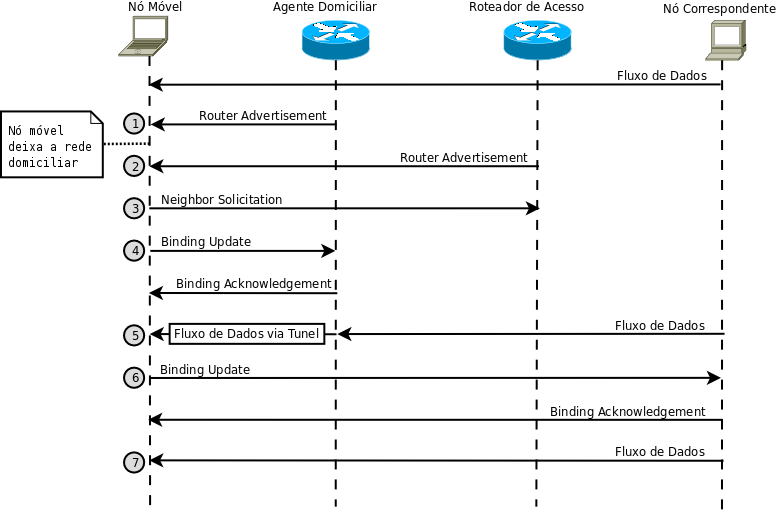
\includegraphics[scale=.37]{figs/fluxo_mipv6}
	\caption{Diagrama de sequencia do MIPv6}
	\label{f_messages}
\end{figure}

Ap�s o fluxo de dados estabelecido, ocorrem as seguintes trocas de mensagens:
\begin{enumerate}
 \item Inicialmente, o n� m�vel recebe uma mensagem de RA do roteador de acesso
da rede domiciliar. O n� compara os
prefixos de seu endere�o domiciliar e o prefixo do endere�o IP divulgado
pelo roteador de acesso e observa que est� na sua rede domiciliar;
 \item At� ent�o o n� m�vel estava trocando mensagens com o n� correspondente
em sua rede domiciliar. Quando seu ponto de acesso muda, o movimento �
detectado atrav�s da mensagem de RA do roteador de
acesso da rede visitada;
 \item Com as informa��es recebidas na mensagem do roteador, o n� m�vel � capaz
de gerar o seu CoA. Ele efetua, ent�o, o teste de
duplicidade de endere�o com as mensagens de \ac{NS};
 \item Com o sucesso do DAD, o n� m�vel faz o registro com o seu agente
domiciliar, enviando o BU  e recebendo como resposta um BA;
 \item A partir deste ponto, o fluxo de dados entre o n� m�vel e o n�
correspondente � realizado atrav�s do tunelamento bidirecional, via Agente
Domiciliar;
 \item Para otimizar o roteamento, o n� m�vel faz o registro do
seu CoA com o n� correspondente. Assim, a comunica��o entre
eles se d� de forma normal, sem a necessidade de encaminhar os pacotes ao agente
domiciliar;
 \item O fluxo de dados � conduzido diretamente ao n� m�vel tendo como endere�o
destino o CoA. O endere�o domiciliar � conduzido no
cabe�alho de mobilidade do IPv6 (\textit{Mobility Header}).
\end{enumerate}

\subsection{Mensagens do MIPv6}
\label{sub_mipv6_mes}
O MIPv6 define um novo cabe�alho de extens�o ao protocolo IPv6,
o \textit{Mobility Header}. Este cabe�alho de mobilidade � utilizado pelos n�s
m�veis e correspondentes, bem como pelo agente domiciliar, para construir as
mensagens utilizadas no MIPv6.

As mensagens enviadas utilizando o cabe�alho de mobilidade s�o as seguintes:
\begin{enumerate}
 \item \textbf{\textit{Binding Refresh Request} (BRR)}: mensagem enviada
pelos n�s correspondentes ao n� m�vel, para requisitar a atualiza��o do registro
de mobilidade;
 \item \textbf{\textit{Home Test Init} (HoTI)}: mensagem enviada pelo n� m�vel
para o n� correspondente, via agente domiciliar, utilizada para iniciar o
procedimento de \textit{Return Routability}. Requisita o \textit{home keygen
token}. utilizado pelo n� m�vel para gerar a chave \textit{Kbm};
 \item \textbf{\textit{Care-of Test Init} (CoTI)}: mensagem envianda pelo n�
m�vel para o n� correspondente, pertencente ao processo de
\textit{Return Routability}. Requisita o \textit{care-of keygen token} utilizado
pelo n� m�vel para gerar a chave \textit{Kbm};
 \item \textbf{\textit{Home Test} (HOT)}: mensagem em resposta ao HoTI enviada
pelo n� correspondente ao n� m�vel;
 \item \textbf{\textit{Care-of Test} (COT)}: mensagem em resposta ao CoTI
enviada pelo n� correspondente ao n� m�vel;
 \item \textbf{Binding Update}: mensagem utilizada para notificar o agente
domiciliar e os n�s correspondentes, do novo CoA;
 \item \textbf{Binding Acknowledgement}: mensagem utilizada para confirmar o
\textit{Binding Update};
 \item \textbf{Binding Error}: mensagem enviada pelos n�s correspondentes ao n�
m�vel, para informar erro na mobilidade relatada.
\end{enumerate}

\subsection{Considera��es sobre Seguran�a}
\label{sub_mipv6_secure}
O uso de \acp{BU} n�o autenticados � tido como um s�rio problema
de seguran�a, pois, um n� mal intencionado pode forjar um registro com o n�
correspondente e passar a receber os pacotes destinados ao n� m�vel. Com a
inten��o de solucionar este problema de seguran�a \cite{rfc3776}, o protocolo
MIPv6 implementa alguns mecanismos.

Para dar mais prote��o no processo de BU com o Agente
Domiciliar pode se utilizar o protocolo \ac{IPSec} nativo no IPv6. A troca de
mensagens � feita utilizando um dos cabe�alhos de seguran�a:
\begin{itemize}
 \item \ac{AH} \cite{rfc2402}: representa
um cabe�alho de extens�o do protocolo IPv6 e foi criado para
indentificar/autenticar os pontos comunicantes.
 \item \ac{ESP} \cite{rfc2406}:
representa um cabe�alho de extens�o do protocolo IPv6 que fornece integridade e
confidencialidade aos datagramas IP por meio da cifra dos dados contidos no
datagrama.
\end{itemize}

Para o uso de um dos cabe�alhos de seguran�a � necess�rio um relacionamento
pr�vio de seguran�a entre o n� m�vel e o agente domiciliar, ou seja, uma chave
secreta deve ser configurada nos dois n�s.

No processo do registro do n� m�vel com o n� correspondente torna-se imposs�vel
utilizar o IPsec para prover seguran�a no processo, pois o n� correspondente
pode ser estar localizado em qualquer lugar na \textit{Internet} e uma chave
secreta n�o pode ser pr�-configurada. Para tornar o processo seguro faz-se
necess�rio o uso de algum mecanismo global de autentica��o autom�tica. A solu��o
proposta para esse problema � conhecida como \ac{RRP}.

\subsubsection{\textit{Return Routability Procedure}}
\label{sub_sub_mipv6_rrp}
Na tentativa de tornar mais seguro o registro do n� m�vel com o n�
correspondente o MIPv6 introduz o RRP
\cite{rfc3775}. A id�ia do processo � que o n� correspondente obtenha garantias
de que o n� m�vel seja alcan��vel pelo seu endere�o domiciliar e pelo seu
CoA. Somente assim o n� correspondente estar� apto para
receber \acp{BU}.

O teste \cite{rfc4225} consiste em enviar, a partir do n� m�vel, duas mensagens
ao n� correspondente: uma via agente domiciliar (\textit{Home Test Init}) e
outra diretamente ao n� correspondente (\textit{Care-of Test Init}). Em resposta
o n� correspondente envia duas mensagens (\textit{Home Test} e \textit{Care-of
Test}). A partir dos dados destas mensagens o n� m�vel � capaz de gerar uma
chave de seguran�a denominada \textit{binding management key} (Kbm).

Na figura \ref{f_rrp} pode-se observar o fluxo das mensagens utilizados
no RRP.
\begin{figure}[!htpb]
	\centering
	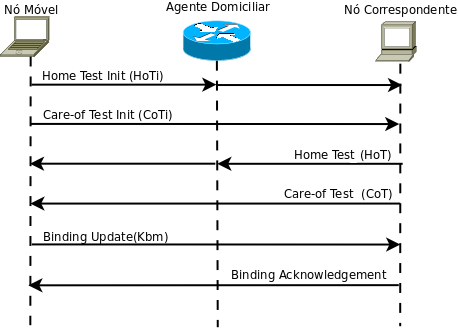
\includegraphics[scale=.5]{figs/rrp}
	\caption{Fluxo das mensagens no Return Routability Procedure}
	\label{f_rrp}
\end{figure}

Para autorizar o BU o n� m�vel gerou a chave \textit{Kbm} 
que permite uma verifica��o por parte do n� correspondente. Ao receber o BU o n�
correspondente � capaz de recalcular a Kbm e permitir a associa��o do CoA com o
endere�o domiciliar.

� importante salientar que o RRP n�o � totalmente seguro, pois um atacante pode
capturar as mensagens enviadas pelo n� correspondente e forjar mensagens de
\acp{BU}. Obviamente o mesmo atacante conseguir� fazer o mesmo
ataque em uma rede IPv6 sem mobilidade. Pode-se concluir que o RRP n�o
introduz riscos adicionais ao protocolo IPv6 b�sico.


\section{Vis�o geral do protocolo HMIPv6}
\label{s_hmipv6}
O modelo do protocolo MIPv6 apresenta alguns problemas que comprometem a sua
escalabilidade na \textit{Internet}, alguns desses puderam ser observados nos
cen�rios estudados neste trabalho. Dentre estes problemas podemos destacar:
\begin{itemize}
 \item tempo na detec��o do movimento;
 \item tempo na configura��o do novo endere�o na rede visitada, o CoA;
 \item tempo do registro com o seu Agente Domiciliar;
\end{itemize}

Em um ambiente utilizando o MIPv6 com um excessivo numero de n�s m�veis a
tend�ncia � que se tenha perda na qualidade de servi�o e o aumento do
\textit{delay} na entrega dos pacotes.

Com o intuito de minimizar os efeitos dos longos retardos no envio dos
\acp{BU}, para o registro com o Agente Domiciliar ou com os n�s
correspondentes e, reduzir o tr�fego de pacotes de controle na
\textit{Internet}, foi proposto um protocolo complementar ao MIPv6, o 
\acf{HMIPv6} \cite{rfc4140}.

%ref
A id�ia principal do protocolo � tratar a mobilidade global e local de formas
distintas. Uma movimenta��o local pode ser entendida como a que acontece dentro
de um mesmo dom�nio e a global entre dom�nios diferentes.
Podemos definir um dom�nio como uma dimens�o arbitr�ria, por exemplo,
uma rede de uma empresa ou universidade com uma ou mais subredes.

Um estudo \cite{kirby1995lu} sobre os padr�es de mobilidade analisou diversos
profissionais, mostrou que 69\% das movimenta��es s�o locais independente deles
possu�rem algum dispositivo m�vel. Este dado mostra que o modelo hier�rquico �
mais adequado para o uso na \textit{Internet}. As principais vantagens seriam a
diminui��o no tempo do \textit{handover} e do tr�fego de sinaliza��o enviado
para � \textit{Internet}.

\subsection{Funcionamento do HMIPv6}
\label{sub_func_hmipv6}
A principal mudan�a no HMIPv6 em rela��o ao MIPv6 foi � introdu��o de um novo
agente, o \ac{MAP}, que nada mais � do que um roteador utilizado para gerenciar
a mobilidade em um determinado dom�nio. O funcionamento do Agente
Domiciliar e dos n�s correspondentes permanece id�ntico ao do MIPv6. Assim como
no MIPv6, o funcionamento do HMIPv6 n�o depende da tecnologia de acesso.

Quando um n� movel entra em um dom�nio com a presen�a de um MAP, ele
ir� receber uma mensagem RA com informa��es sobre os roteadores de acesso. Isso
permite que ele autoconfigure dois endere�os: o \ac{RCoA}, que ser�
baseado em um prefixo de uma rede do MAP, e o \ac{LCoA}, que utilizar� o
mesmo prefixo anunciado pelo roteador padr�o.

Ap�s gerar os endere�os RCoA e LCoA, o n� m�vel ir� atualizar suas associa��es.
Ele enviar� um \textit{Binding Update} para o MAP, para que este fa�a a
associa��o do RCoA com o LCoA. Outros \acp{BU} tamb�m ser�o
enviados para o Agente Domiciliar e, opcionalmente, para os n�s correspondentes.
Neste caso, para que estes fa�am a associa��o do endere�o domiciliar com o RCoA.
Se o n� m�vel estiver se comunicando com correspondes locais, ou seja, do mesmo
dom�nio, ele deve enviar um BU para � associa��o do endere�o domiciliar com o
LCoA.

O funcionamento do MAP � semelhante ao do Agente Domiciliar: ele intercepta
pacotes destinados ao RCoA, originados pelo tunelamento entre Agente
Domiciliar e n� m�vel, ou pelos pacotes provindos diretamente dos n�s
correspondentes. Neste �ltimo caso, o destino dos pacotes provindos dos n�s
correspondentes � o RCoA, sendo que o endere�o domiciliar � colocado no
cabe�alho de mobilidade do IPv6. Seja qual for o caso, o MAP envia os pacotes
destinados ao RCoA pelo t�nel bidirecional, estabelecido entre o MAP
e o LCoA. Este t�nel � tamb�m usado para enviar todos os pacotes oriundos do n�
m�vel, exceto os com destino aos correspondentes locais.

Dois comportamentos podem ser distinguidos no protocolo HMIPv6: quando o n�
m�vel se desloca dentro de um mesmo dom�nio (mobilidade local) e entre dom�nios 
diferentes (mobilidade global):
\begin{description}
 \item[Mobilidade local:] quando o n� m�vel muda somente o seu endere�o LCoA,
ou seja, muda de roteador de acesso mas continua sob a cobertura do mesmo MAP.
Neste caso, � necess�rio o envio de \acp{BU} para o MAP e os
correspondentes
locais, atualizando a associa��o RCoA-LCoA. Como resultado, os pacotes com
origem no agente domiciliar e nos n�s
correspondentes continuar�o a serem enviandos para o mesmo RCoA, minimizando o
tempo do \textit{handover} e a perda de pacotes. Tamb�m notamos que todo tr�fego
gerado � dentro do mesmo dom�nio.

\item[Mobilidade global:] neste caso o n� m�vel reconfigura o seu RCoA e LCoA, e
envia \acp{BU} para o MAP, os n�s comunicantes fora do dom�nio
informando o novo RCoA e os n�s do mesmo site para informar o LCoA.
\end{description}

A figura \ref{f_hmipv6} ilustra um exemplo de dom�nios HMIPv6 onde o n� m�vel
est� inicialmente atrelado a rede domiciliar. Em seguida, realiza mobilidade
para o \textit{dom�nio 1}, tendo como roteador padr�o o RA1, e utilizando o
MAP1. Ap�s isso, o n� m�vel realiza uma mobilidade local, mudando o roteador
padr�o para RA2. Por �ltimo, realiza uma mobilidade global, passando a ter o RA3
como roteador padr�o, e passando a utilizar o MAP2.

\begin{figure}[!htpb]
	\centering
	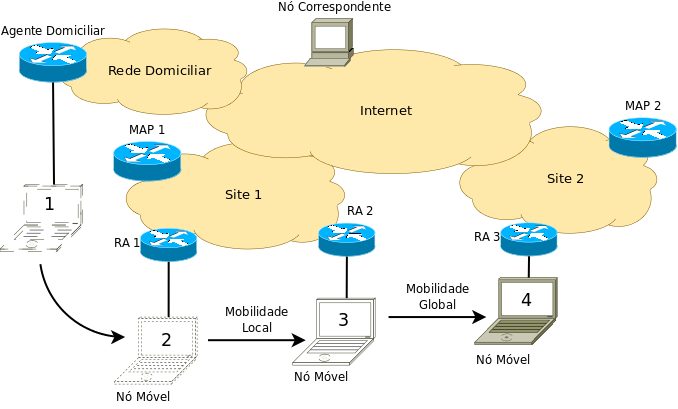
\includegraphics[scale=.45]{figs/hmipv6}
	\caption{Exemplo de dom�nios do IP M�vel Hier�rquico}
	\label{f_hmipv6}
\end{figure}

A figura \ref{f_messages_hmipv6} apresenta a sequ�ncia de mensagens trocadas
durante o movimento do n� m�vel no cen�rio da figura \ref{f_hmipv6}, sendo
suprimido os processos de DAD e RRP.

\begin{figure}[!htpb]
	\centering
	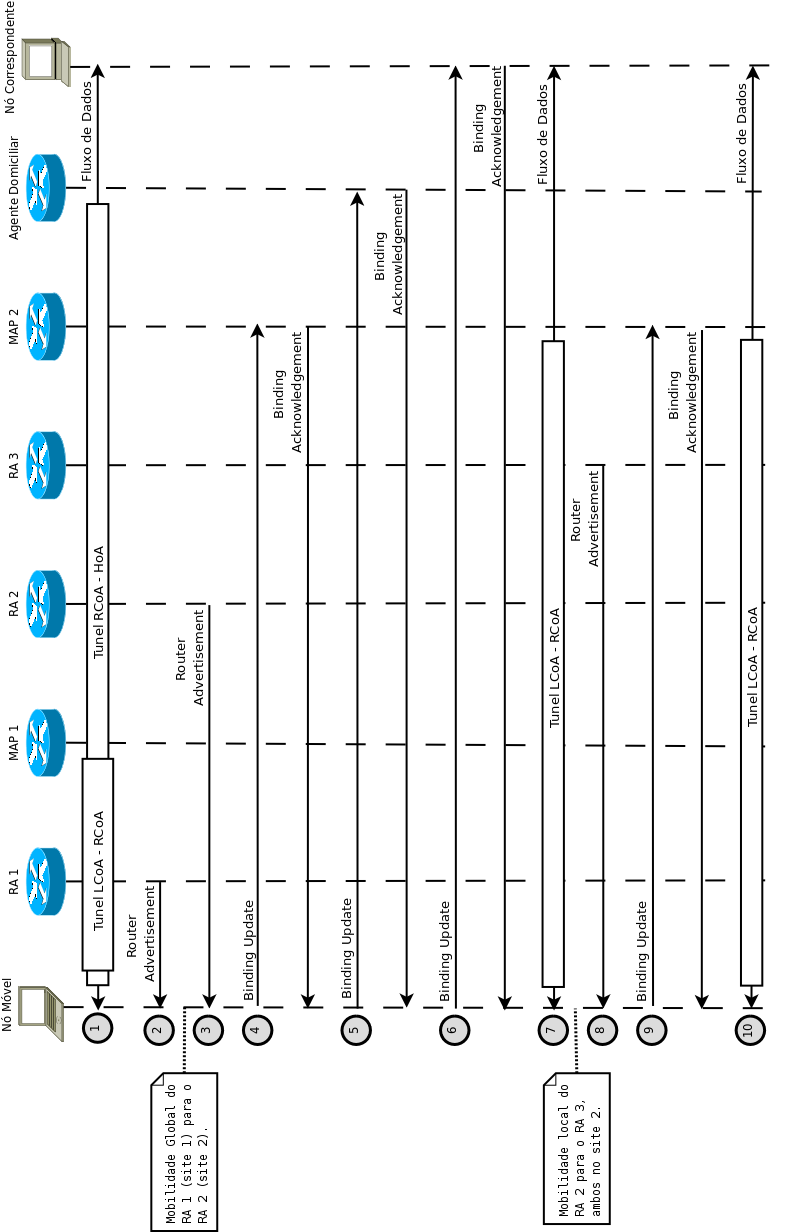
\includegraphics[scale=.36]{figs/fluxo_hmipv6}
	\caption{Diagrama de troca de mensagens do HMIPv6}
	\label{f_messages_hmipv6}
\end{figure}

As trocas de mensagens que ocorrem na figura \ref{f_messages_hmipv6}
s�o descritas a seguir:

\begin{enumerate}
 \item Inicialmente o n� m�vel est� na rede domiciliar se comunicando com o um
correspondente.
 \item O MAP1 envia mensagens de RA. Os
roteadores de acesso RA1 e RA2, sob a cobertura de MAP1, ir�o anexar as
informa��os recebidas das mensagens RA do MAP 1 e, encaminhar para suas
subredes, via RA. O n� m�vel recebe uma mensagem de RA do RA1, realizando
a mobilidade para a respectiva rede;
 \item O n� m�vel realizar� o registro com o MAP1, enviando-lhe um BU,
associando desta forma o endere�o domiciliar com o
LCoA1. Ap�s efetuar o registro, o MAP1 enviar� um BA;
 \item O pr�ximo n� com quem o n� m�vel realizar� o registro ser� o agente 
domiciliar. A diferen�a ser� que o registro ir� associar o endere�o domiciliar
com o RCoA1;
 \item O fluxo de dados percorre o seguinte caminho: sai do n� correspondente
com destino ao endere�o domiciliar. Como o n� movel n�o est� na rede domiciliar,
o Agente Domiciliar interceptar� os pacotes, e encaminhar� para o endere�o
registrado, via t�nel, no caso o RCoA1. Quando chegar no MAP1, ser� tunelado
novamente at� o LCoA1. O fluxo de dados passa pelo RA1, mas ele s� encaminha o
pacote para o n� m�vel, onde termina os t�neis;
 \item O n� m�vel se movimenta e sai do alcance do RA1 e entra na cobertura
de RA2. Como foi feita uma mobilidade local, ser� neccess�rio somente configurar
um novo LCoA (LCoA2);
 \item Ser� necess�rio atualizar o registro com o MAP1, associando o
LCoA2 ao endere�o domiciliar. N�o � necess�rio novo registro com o MAP1;
 \item O trajeto do fluxo de dados ser� alter�do do MAP1 para frente, sendo
transparente para o n� correspondente e para o Agente Domiciliar. O t�nel entre
o MAP1 e o n� m�vel ter� como destino o LCoA2, e passar� pelo RA2, o roteador
padr�o do n� m�vel.
 \item O n� m�vel recebe uma mensagem RA com informa��es de um outro MAP
atrav�s do RA3, o que indica que ocorreu uma mobilidade global est� em
andamento. Um novo LCoA ser� formado (LCoA3) e um novo RCoA(RCoA2);
 \item O primeiro registro ser� com o novo MAP, o MAP2. A associa��o feita ser�
do endere�o domiciliar com o LCoA3;
 \item O registro no Agente Domiciliar ser� atualizado, associando o
endere�o domiciliar com o RCoA2;
 \item O registro com o n� correspondente � realizado, associando o endere�o
domiciliar com  RCoA2. Ap�s o registro, o agente domiciliar ser� utilizado
somente por outro correspondente para encontrar o n� m�vel e estabelecer uma
comunica��o;
 \item O fluxo de dados ser� endere�ado ao RCoA2, e utilizar� um cabe�alho 
de mobilidade, indicando que o pacote � endere�ado ao endere�o domiciliar do n�
m�vel.
\end{enumerate}

Podemos perceber que, em algumas vezes o n� m�vel deve preferir atuar como no
MIPv6 para tornar mais simples o seu funcionamento. Neste caso a rede visitada
se encontra pr�xima ao agente domiciliar e n�o se faz necess�rio o uso do MAP.

\subsection{Envio de \textit{Binding Updates}}
%ref
Ap�s o evento de mobilidade global, o n� m�vel autoconfigura um novo RCoA e um
novo LCoA e ele precisa enviar um BU para o MAP. O BU ir� associar o RCoA com o
LCoA, de forma similar
a associa��o do CoA com o endere�o domiciliar no MIPv6. O MAP far� o DAD do
RCoA, somente no primeiro BU, e
retornar� um BA para o n� m�vel.

A especifica��o do protocolo permite que um n� m�vel tenha mais de um RCoA.
Isto se aplica para o caso deste ter recebido mais de uma op��o de MAP. Nesta
situa��o, dever� ser feito um Binding Update para cada RCoA . 

Depois de fazer o registro com o MAP o n� m�vel deve fazer a associa��o do RCoA
com o endere�o domiciliar no agente domiciliar e nos n�s correspondentes. A
mensagem de BU deve ser envianda utilizando a op��o de
CoA alternativo preenchida com o RCoA e o tempo de vida
deve ser menor que o do recebido no BA do registro
com o MAP.

\subsection{Descoberta de um MAP}
O n� m�vel e os roteadores de acesso deve obter de alguma forma o endere�o do
e o prefixo de rede do MAP. Dois m�todos s�o definidos para o descobrimento do
MAP:
 
\begin{description}
\item[Descobrimento din�mico:] � baseado na propaga��o da op��o de MAP nas
mensagens de \acp{RA}. Na op��o de MAP est�o presentes o
endere�o global do MAP, seu prefixo de rede e um vetor de dist�ncia baseado nos
saltos da mensagem at� a chegada no n� m�vel. Esta �ltima op��o influenciar� na
escolha do MAP padr�o, e um MAP particular como prefer�ncia. Neste m�todo, os
roteadores de acesso devem ser configurados para receberem as mensagens com
op��es de MAP e as re-enviarem, incrementando o vetor de dist�ncia;
\item[Configura��o manual:] neste m�todo, a op��o de MAP � configurada
manualmente nos roteadores de acesso, por um administrador da rede. Em muitos
dom�nios esse � o mescanismo padr�o.
 \end{description}

% ----------------------------------------------------------------------- %
% Arquivo: plataformadetestes.tex
% ----------------------------------------------------------------------- 

\chapter{Plataforma de Testes para Mobilidade em Redes IP}
\label{c_plataforma}

\section{Descri��o Geral da Plataforma}
\label{s_plataforma_intro}

A plataforma desenvolvida neste trabalho tem como objetivo prover o usu�rio com:
\begin{itemize}
 \item um sistema que permita facilidades no estudo dos protocolos de
mobilidade da camada de rede, em particular o MIPv6 e HMIPv6. Outros protocolos
poder�o ser instalados no futuro;
 \item facilidades para a r�pida constru��o de cen�rios de rede, sem se ater a
procedimentos de configura��o e instala��o de equipamentos de rede sem fio;
\item facilidades para a r�pida instala��o da platfaorma nas m�quinas
hospedeiras;
\end{itemize}

Na concep��o da plataforma de testes, optou-se por utilizar um ambiente baseado
em m�quinas virtuais devido a rapidez na realiza��o de experimentos: em somente
uma m�quina de hospedagem � poss�vel o desenvolvimento, an�lise e testes de
protocolos de rede. Al�m disto, existem vantagens econ�micas e de redu��o de
complexidade, pois n�o h� necessidade de diversos equipamentos para a realiza��o
dos experimentos.

Em geral, uma plataforma de testes de mobilidade envolve o uso de redes sem fio.
No entanto, como o objetivo principal da plataforma � possibilitar o estudo de
protocolos de camada 3, decidiu-se por construir um ambiente de teste atrav�s de
m�quinas virtuais linux em modo usu�rio - UML \cite{uml09}
adaptando os \textit{switches} virtuais para produzir a mobilidade. Desta forma,
evita-se a complexidade adicional de instala��o de hardware para a rede sem
fio.

Os seguintes componentes podem ser identificados nesta plataforma:
\begin{itemize}
 \item m�quinas e \textit{switches} virtuais UML para constru��o de dom�nios e
dos n�s m�veis. Os \textit{switches} virtuais foram modificados para a simula��o
de mobilidade;
\item Interface gr�fica para permitir a r�pida constru��o de cen�rios e para
possibilitar o comando de mobilidade.
\item Ferramentas para estudo dos protocolos: gerador de tr�fego, medidor de
banda e de perda de pacotes;
\item Protocolos de Mobilidade da Camada 3: instala��o, nas UMLs, de uma vers�o
do IPv6 m�vel, do gerador de mensagens de advert�ncia de roteador
do IPv6 (RADVD) e de uma vers�o do HMIPv6. Como ser� visto adiante, n�o existe
uma vers�o atualizada do protocolo HMIPv6. Parte do trabalho foi dedicada a uma
extens�o do MIPv6 para o HMIPv6;
\item Outros protocolos e ferramentas de apoio: alguns protocolos e
ferramentas adicionais foram instalados, tais como o protocolos RIP e o
protocolo OSPF, atrav�s do pacote Zebra \cite{Zebra09}
\end{itemize}

Na sequ�ncia, apresentamos alguns detalhes sobre os componentes da plataforma
sendo que os aspectos relacionados aos protocolos de mobilidades ser�o
discutidos separadamente nos pr�ximos cap�tulos.


\section{A UML como Bloco B�sico da Plataforma de Testes}

\subsection{UML - \textit{Linux} em Modo Usu�rio}
\label{s_plataforma_uml}

A m�quina virtual \textit{Linux} em Modo Usu�rio (\textit{User Mode Linux} -
UML) foi escolhida como base para a constru��o das redes virtuais na plataforma
de testes. Ela oferece v�rias possibilidades de constru��o de redes, al�m de ser
incorporada ao \textit{kernel} do Linux e de apresentar um alto desempenho na
execu��o de programas. Isto permite iniciar multiplas inst�ncias UML em uma
mesma m�quina hospedeira e a constru��o de complexos cen�rios de rede.

O Linux executa a m�quina UML como um processo comum no sistema. O processo �
executado em um ambiente isolado protegendo a camada f�sica da m�quina
hospedeira, o que n�o imp�e restri��es de uso para a m�quina virtual, tornando
um ambiente excelente para testes \cite{artigo_uml}. A figura
\ref{f_plataforma_uml} mostra o
funcionamento do Linux em Modo Usu�rio em uma m�quina hospedeira.

\begin{figure}[!htpb]
    \centering
    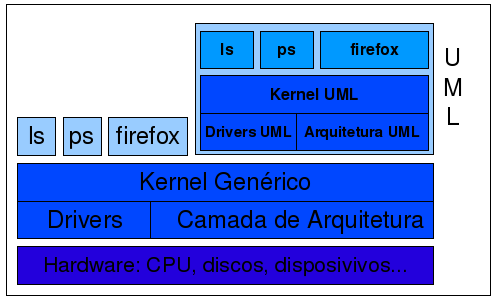
\includegraphics[scale=1]{figs/uml}
    \caption{Funcionamento do Linux em Modo Usu�rio}
    \label{f_plataforma_uml}
\end{figure}

� comum chamar a UML de m�quina virtual, por�m, a tecnologia de virtualiza��o
UML constitue-se, na verdade, em um sistema operacional virtual. O termo
m�quina virtual seria mais aplic�vel em tecnologias de virtualiza��o tal como a
\textit{VMWare}, onde realmente � emulada uma plataforma
f�sica, processador e perif�ricos, sendo que o sistema operacional � executado
nesta plataforma emulada.

A UML permite construir sistemas que em um ambiente real seriam muito dif�ceis
de reproduzir, por exemplo, � poss�vel criar uma m�quina com \textit{n}
interfaces de rede e discos. Devido a sua flexibilidade, a UML pode ser
utilizada para in�meras aplica��es tais como:
\begin{itemize}
 \item Consolida��o de servidores de rede: � possivel reproduzir todo sistema em
UML e test�-lo antes de coloc�-lo em produ��o;
 \item Em ambientes de ensino: com UML os alunos podem desenvolver as atividades
ensinadas sem a preocupa��o de danificar o sistema;
 \item No desenvolvimento de aplica��es em n�vel usu�rio, protocolos de rede, do
\textit{kernel linux};
\end{itemize}

Para utilizar a UML � preciso um \textit{kernel} Linux compilado para a
arquitetura \textit{um} e um sistema de arquivos, que nada mais � do que um
simples arquivo contendo a imagem de um sistema, onde temos toda a estrutura de
diret�rios e os demais componentes para uma execu��o normal de um Linux. A UML
realiza as opera��es de escrita e leitura de arquivos no sistema de arquivos,
analogamente ao que sistema hospedeiro realiza no disco r�gido.

Para esta plataforma de testes, o \textit{kernel} linux-2.6.27 foi compilado com
v�rios recursos de rede. Um sistema de arquivos foi constru�do a partir da
distribui��o \textit{GNU/Linux Debian Lenny}. A id�ia foi construir um pequeno
sistema dedicado para laborat�rios de redes. Ele inclui as implementa��es dos
protocolos de rede e um conjunto de utilit�rios para solucionar problemas de
rede.

Os principais componentes e recursos de rede dispon�veis no \textit{kernel}
compilado e no sistema de arquivos s�o:
\begin{itemize}
 \item Implementa��es do MIPv6 e HMIPv6;
 \item Implementa��es dos protocolos de roteamento RIPv2, RIPng, OSPFv2, OSPFv3
e BGP4;\begin{large}       \end{large}
 \item Utilit�rios de rede: \textit{tcpdump}, \textit{ping}, \textit{ping6},
\textit{traceroute}, \textit{ip}( mostra e manipula rotas, dispositivos,
policita de roteamento e tunels), \textit{iptables}, \textit{tc};% (citar mais)
 \item Ferramentas IPSec;
 \item \textit{Kernel} suporte para \textit{Netfilter};
 \item \textit{Kernel} suporte para Qualidade de servi�o (QoS);
 \item \textit{Kernel} suporte para IP Seguro (IPSec) pra IPv4 e IPv6;
 \item \textit{Kernel} suporte a mobilidade e otimiza��o de roteamento em redes
IPv6;
\end{itemize}

Outros componentes e recursos podem facilmente ser adicionados a plataforma de
testes.

\subsection{Redes Virtuais M�veis com a m�quina UML}

UML oferece dois tipos de redes para as maquinas virtuais: uma que permite
conectar a UML com o hospedeiro e uma outra denominada redes virtuais isoladas
onde somente fazem parte inst�ncias UML. No primeiro tipo de rede as tecnologias
de transporte utilizados pela UML s�o: \textit{TUN/TAP}, \textit{Ethertap},
\textit{SLIP} e \textit{Slirp}. No segundo tipo: \textit{switch} virtual e
\textit{Multicast}.

Nos cen�rios de rede, para testes dos protocolos de rede, foram utilizadas as
redes virtuais isoladas. O programa \textit{uml\_switch}, integrante do pacote
UML, permite a interliga��o
das m�quinas virtuais. Ele � um utilit�rio que implementa um \textit{switch
Ethernet} ou um \textit{hub} em \textit{software}. As m�quinas UML se conectam
ao \textit{switch} e se comunicam por meio de um arquivo de dom�nio \textit{UNIX
sockets} no hospedeiro.

Na figura \ref{f_plataforma_vnuml} observamos as duas formas de redes virtuais
UML. Note que a flexibilidade da m�quina virtual permite � inst�ncia UML
participar das duas redes.

\begin{figure}[!htpb]
    \centering
    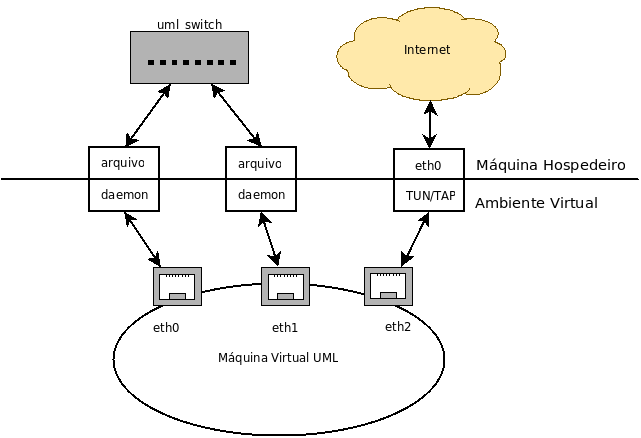
\includegraphics[scale=.6]{figs/vnuml}
    \caption{Redes Virtuais UML}
    \label{f_plataforma_vnuml}
\end{figure}

Em geral, uma plataforma de testes de mobilidade envolve o uso de redes sem fio,
contudo os protocolos estudados s�o em n�veis de camada 3 sendo a mudan�a de
portas em um \textit{switch} suficiente para verificar boa parte do
comportamento dos protocolos.  Tornou-se necess�rio ent�o fazer altera��es no
programa do \textit{uml\_switch}, que � um software livre sobre a licen�a GPL
vers�o 2, escrito na linguagem de programa��o C. 

A principal altera��o no c�digo fonte do \textit{uml\_switch} foi a inclus�o da
possibilidade de segmenta��o de redes, permitindo a cria��o de uma esp�cie de
\textit{VLan}. Desta forma � poss�vel realizar a mobilidade dos n�s conectados
ao \textit{switch}. Ap�s a mudan�a, cada n� conectado ao \textit{switch}
pertence a uma \textit{VLan} e � poss�vel mover o n� para outra \textit{VLan}.

Outra implementa��o que foi realizada no \textit{uml\_switch} foi a adi��o de
uma \textit{thread} que responde um servidor \textit{telnet}, que basicamente
tem duas fun��es. A primeira � permitir o usu�rio efetuar a mobilidade dos
n�s conectados no \textit{switch}. A outra fun��o, � listar os n�s conectados.
Esse recurso torna f�cil a implementa��o de uma interface gr�fica do
\textit{switch}, pois um outro programa, em outra linguagem de programa��o, pode
utilizar-se deste recurso para gerar a interface.

%\section{MobUML - }

\section{GUML4MIP - Interface Gr�fica de controle de terminais UML para o IP M�vel}
A m�quina virtual UML tem se mostrado uma �tima ferramenta para a plataforma
de teste. Por�m, a sua utiliza��o na constru��o de redes virtuais n�o � muito
pr�tica, porque para cada cen�rio � necess�rio a cria��o de \textit{scripts}
para iniciar as m�quinas e configurar as redes. Isto torna a constru��o de
cen�rios demorada e n�o t�o evidente, al�m do fato de que o usu�rio necessita de
bons conhecimentos do sistema operacional \textit{linux}, indo um pouco contra a
id�ia proposta pela plataforma.

Pelo motivo apontado teve-se a id�ia de construir uma interface gr�fica,
amig�vel para o usu�rio, de forma a possibilitar: a constru��o r�pida de
cen�rios com
redes, o controle da mobilidade dos n�s e a centraliza��o de todos os terminais
das m�quinas virtuais em uma �nica janela. Esta �ltima carater�stica evitaria
que, em cen�rios muito complexos, um grande n�mero de janelas
fossem abertas, diminuindo a produtividade durante sua utiliza��o.

Ap�s algumas pesquisas na \textit{internet} foi encontrado o projeto de c�digo
aberto ``Interface Gr�fica para controle de terminais UML'' (GUML), feito com a
linguagem de programa��o \textit{Python} e que j� contempla muitos dos recursos
pretendidos. Decidiu-se fazer altera��es no c�digo fonte deste projeto de forma
a implementar os novos recursos pretendidos.

Como citado, apesar de possuir v�rios recursos, o GUML n�o prov� suporte a
configura��o de cen�rios de rede integrado na ferramenta. E seu intuito n�o �
ser uma interface para constru��o de cen�rios de redes m�veis e sim para controle de
terminais UML. Por esse motivo optou-se fazer um \textit{fork} do projeto e
criar um outro um chamado ``Interface Gr�fica de controle de terminais UML para o IP M�vel'' 
(GUML4MIP), baseado-se no seu c�digo fonte.

Os principais recursos incorporados ao GUML4MIP, que possibilitam e melhoram 
o suporte as redes virtuais, s�o:

\begin{itemize}
 \item Adi��o de par�metros no arquivo de configura��o passando a ser
poss�vel especificar:
\begin{itemize}
 \item A fun��o da m�quina UML: um roteador ou um n� hospedeiro;
 \item Endere�o IP das interfaces das m�quinas UML;
 \item A \textit{VLan} que a interface da m�quina UML ser� atrelada;
 \item Servi�os adicionais que poder�o ser iniciados \textit{boot} da m�quina
UML. Por exemplo, o \textit{daemon} do \textit{mipl} ou do \textit{radvd};
\end{itemize}
 \item Gera��o autom�tica de \textit{scripts} de configura��o de rede;
 \item Roteamento din�mico utilizando o \textit{Zebra};
 \item Possibilidade de carregar novos cen�rios de rede em tempo de execu��o da interface;
 \item Interface gr�fica do \textit{uml\_switch} (ver figura \ref{f_plataforma_gswitch}),
com este recurso o usu�rio pode visualizar o estado do \textit{uml\_switch} durante a 
execu��o do cen�rios;
 \item Controle da mobilidade das m�quinas UML por meio da interface do \textit{uml\_switch}.
\end{itemize}

Acompanha o pacote do GUML4MIP um aplicativo, chamado \textit{create\_fs}, que constr�i
automaticamente o sistema de arquivos especificado neste cap�tulo para a plataforma
de testes.

Para utilizar o GUML4MIP o usu�rio deve configurar um arquivo para cada m�quina UML.
No arquivo de configura��o � poss�vel configurar: 
\begin{itemize}
 \item O sistema de aquivo que a m�quina virtual ir� utilizar;
 \item Quantidade de mem�ria para a m�quina virtual;
 \item Interfaces de rede;
 \item Discos;
\end{itemize}

Um exemplo de arquivo de configura��o do GUML4MIP, pode
ser observado no anexo \ref{c_anexo_guml4mip}.

Na figura \ref{f_plataforma_guml} podemos observar o visual da interface,
rodando um cen�rio de rede, e os recursos dispon�veis ao usu�rio. Abaixo 
uma explica��o detalhada das fun��es que o usu�rio pode realizar na interface:
\begin{figure}[!htpb]
	\centering
	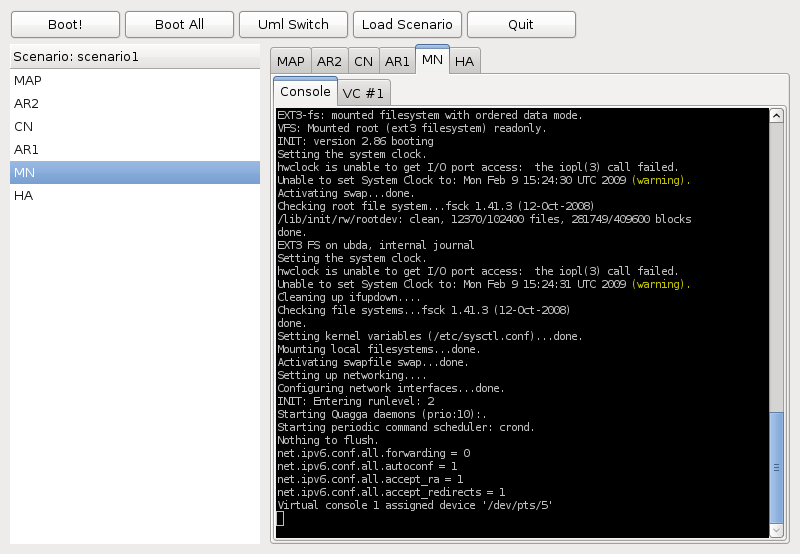
\includegraphics[scale=.55]{figs/guml4mip}
	\caption{Interface Gr�fica de controle de terminais UML para o IP M�vel}
	\label{f_plataforma_guml}
\end{figure}

\begin{description}
  \item[\textit{Boot !}] Clicando neste bot�o o usu�rio inicia a m�quina UML selecionada
no quadro que lista as m�quinas do cen�rio;
  \item[\textit{Boot All}] Este bot�o permite que o usu�rio inicie todas as m�quinas
UML configuradas para o cen�rio, a direita por meio das asbas o usu�rio pode acessar o
terminal das m�quinas virtuais;
  \item[\textit{Uml Switch}] Clicando neste bot�o uma nova janela ser� aberta. Na
janela do \textit{uml\_switch}, figura \ref{f_plataforma_gswitch}, o usu�rio 
pode observar todas as m�quinas virtuais conectados a ele, e a qual \textit{VLan} 
cada interface de rede esta associada. Caso o usu�rio queira efetuar alguma 
mobilidade basta clicar no n�mero da \textit{VLan} a qual queira se associar.
  \item[\textit{Load Scenario}] Por meio deste bot�o o usuario busca o diret�rio
onde est�o os arquivos de configura��o de um novo cen�rio de rede. O ultimo cen�rio
executado � salvo e na proxima execu��o do programa j� � carregado automaticamente.
  \item[\textit{Quit}] Encerra o programa.
\end{description}

%% figuras do guml modificado e do uml switch
\begin{figure}[!htpb]
	\centering
	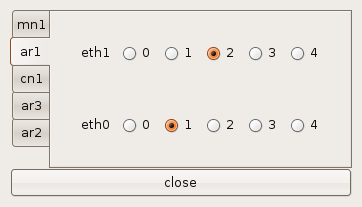
\includegraphics[scale=.6]{figs/uml_switch}
	\caption{Interface Gr�fica para o \textit{uml switch}}
	\label{f_plataforma_gswitch}
\end{figure}

\subsection{Funcionamento do GUML4MIP}

O programa GUML4MIP possui um funcionamento bem simples, por esse motivo se
torna uma aplica��o vers�til e facilmente alter�vel. Na figura \ref{f_plataforma_gfunc}
tentamos exemplificar o seu funcionamento. Em resumo o seu funcionamento pode 
ser descrito nas seguintes etapas:

\begin{enumerate}
 \item Ao iniciar, realiza a leitura dos arquivos de configura��o das m�quinas UML 
no diret�rio do cen�rio a ser executado. Na primeira execu��o do programa o cen�rio
carregado � um exemplo que vem junto com o pacote do GUML4MIP, nas outras execu��es o
�ltimo cen�rio executado � o padr�o. 
 \item A partir dos arquivos de configura��o cria as linhas de comando que executaram
as m�quinas UML e o arquivo \textbf{guml4mip.conf}. Um \textit{script} que configura 
as interfaces de rede das m�quinas UML e os \textit{daemons} para iniciarem.
 \item Inicia o processo do \textit{uml\_switch}, qual as m�quinas UML ir�o se conectar.
Em paralelo uma \textit{thread} � criada e se conecta ao servidor
\textit{telnet} do \textit{uml\_switch}. Por meio desta conex�o, o GUML4MIP monitora
as conex�es no \textit{uml\_switch}, que permitem apresentar em uma interface
gr�fica o estado do \textit{switch} e tamb�m provocar a mobilidade das m�quinas
UML.
 \item Ent�o disponibiliza os recursos do programa ao usu�rio em uma janela constru�da em \textit{PyGTK}.
 \item Ao utilizar fun��o que permite carregar um novo cen�rio, bot�o \textit{Load Scenario}, o programa
encerra os processos das m�quinas do cen�rio anterior, finaliza a conex�o com servidor telnet do \textit{uml\_switch}. O mesmo que quando acionar o bot�o \textit{Quit}, por�m, neste caso reinicia todas
as etapas.
\end{enumerate}

\begin{figure}[!htpb]
	\centering
	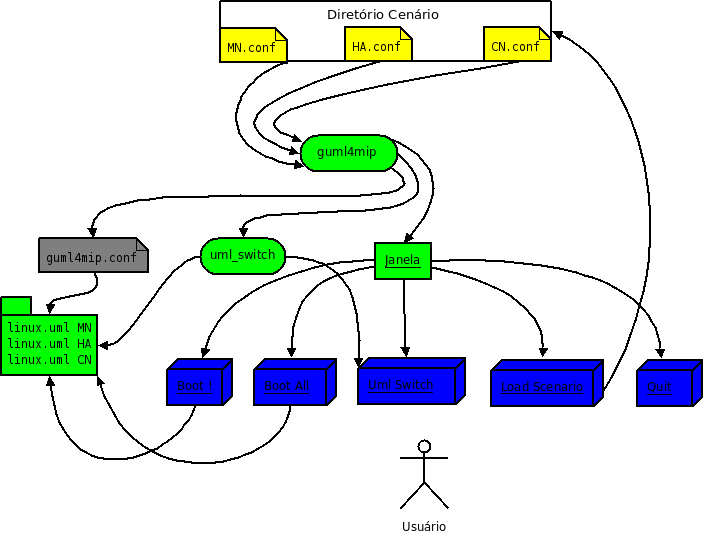
\includegraphics[scale=.6]{figs/guml4mip_func}
	\caption{Funcionamento simplificado do GUML4MIP}
	\label{f_plataforma_gfunc}
\end{figure}

% ----------------------------------------------------------------------- %
% Arquivo: mipl.tex
% ----------------------------------------------------------------------- %
\chapter{Implementa��o do HMIPv6 baseando-se no projeto MIPL}

\section{Implementa��es existentes para Linux dos protocolos de Mobilidade}

O projeto \textit{Mobile IPv6 for Linux} (MIPL) \cite{CitarMIPL} � uma
implementa��o de suporte a mobilidade no IPv6 (RFC 3775), desenvolvida na
Universidade Tecn�logica de Helsinki . O codigo foi desenvolvido acompanhando os
\textit{drafts} da RFC e as vers�es do \textit{kernel linux}. No in�cio do
desenvolvimento, a vers�o do kernel utilizada foi a 2.3.59 e o \textit{draft} 8,
por�m, devido as subst�nciais mudan�as na especifica��o do MIPv6, os gestores 
do projeto decidiram dividir o c�digo fonte uma parte em espa�o de kernel
e outra em espa�o de usu�rio. A �ltima vers�o foi o MIPL 1.1 que trabalhava com
a vers�o 2.4.26 do \textit{kernel linux}.

Mais adiante, iniciou-se o desenvolvimento do MIPL2 pela Universidade de Helsink
juntamente com o projeto USAGI \cite{CitarUsagi}. Nesta nova vers�o houveram
mudan�as significativas: o c�digo foi praticamente todo reescrito e muitas
funcionalidades foram adicionadas em espa�o de usu�rio. Um \textit{daemon}
passou a controlar a sinaliza��o e a detec��o de movimento. A tarefa do
\textit{kernel} passou a ser apenas uma camada de suporte ao MIPv6.

O MIPL2 passou a suportar as �ltimas especifica��es do MIPv6 e passou a utilizar
\textit{framework} XFRM para o suporte a IPSec. � interessante observar tamb�m
que, a partir das �ltimas vers�es do kernel do linux, o suporte ao MIPv6 j� faz
parte da linha principal de desenvolvimento, n�o sendo mais necess�rio aplicar
\textit{patchs}.

No que se refere ao HMIPv6, uma implementa��o foi proposta pela Universidade
de Monash, baseando-se no MIPL 0.94 e na vers�o 2.4 do \textit{kernel linux}.
Tamb�m foram realizadas altera��es no RADVD 0.7.2 para este divulgar mensagens
de MAP. Neste momento, o projeto est� parado e n�o atende mais as necessidades
deste trabalho, pois, ocorreram mudan�as significativas no desenvolvimento do
MIPL. Atualmente a grande maioria dos sistemas j� utilizam a s�rie 2.6 do
\textit{kernel}, ent�o pode-se concluir que n�o h� nenhuma implementa��o
aberta e recente do HMIPv6.

O trabalho prop�e-se, ent�o desenvolver uma  implementa��o experimental
atualizada do HMIPv6, baseando-se na �ltima vers�o est�vel do projeto MIPL
e utilizando a vers�o 0.7.2 do RADVD alterado pelo projeto da Universidade de
Monash.

\section{Estudo do c�digo do projeto MIPL}
Com fins de gerar uma vers�o do HMIPv6 a partir do projeto MIP, iniciou-se
um estudo aprofundado do c�digo fonte do MIPL. O estudo do c�digo do
MIPL2 foi realizado na sua �ltima vers�o est�vel, anunciada pelo projeto USAGI
como umip-0.4. O MIPL � um projeto de codigo aberto sobre a licen�a GPL vers�o
2, escrito na linguagem de programa��o C.

O programa � executado na forma de um \textit{daemon} chamado de \textit{mip6d},
ou seja, um processo executado no segundo plano e que n�o est� associado a um
terminal controlador \ref{stevens}. Este mesmo \textit{daemon} desempenha o
papel de n� m�vel, de agente domiciliar e de n� correspondente. A sua fun��o �
definida em um arquivo de configura��o, sendo que todos os n�s s�o em pontencial
um n� correspondente.

O foco principal do estudo foi na parte respons�vel pelo
funcionamento do n� m�vel, pois as principais mudan�as do MIPv6 para o HMIPv6 �
a funcionalidade deste n�. O agente MAP possui, basicamente, o mesmo
comportamento de um agente domiciliar, a n�o ser pelo de fato de possuir uma
rede com prefixo a partir do qual ser�o criados RCoAs. Al�m do que, todo o
projeto � de alta complexidade, envolvendo o uso de v�rias bibliotecas, o que
demandaria um tempo grande de estudo. � bom lembrar tamb�m que, com fins de
delimitar o escopo do trabalho, foram desconsiderados todos os mecanismos de
seguran�a do HMIPv6.

\subsection{Intera��o entre o \textit{kernel} e o MIPL}
Geralmente tudo o que fizemos, enquanto trabalhamos em um sistema Linux, est�
sendo executado em em espa�o de usu�rio, por exemplo: um editor de texto, um
navegador, servidor X. Em contraste com isso, o \textit{kernel} executa as suas
tarefas em espa�o de \textit{kernel}, com acesso � instru��es privilegiadas,
total controle da mem�ria e do sistema de interrup��es. O principal motivo para
esta separa��o entre dados dos processos do usu�rio e do
\textit{kernel}, � evitar que um perturbe o outro, o que resultaria numa
diminui��o do desempenho, problemas de seguran�a e instabilidades do sistema
\ref{spaces}.

Os motivos levantados acima foram os que levaram os desenvolvedores a passarem a
maioria da implementa��o do protocolo MIPv6 para espa�o de usu�rio, o que torna
desenvolvimento mais f�cil, seguro e independente de vers�o de \textit{kernel}.
Por�m o MIPL precisa de uma interface para a troca de informa��es entre o
\textit{kernel} e espa�o de usu�rio. A troca de informa��o do entre
\textit{kernel} e o espa�o de usu�rio � realizada atrav�s do
\textit{netlink}. O \textit{netlink} consiste em uma extens�o da interface de
soquetes padr�o, que proporciona uma comunica��o bidirecional entre
\textit{kernel} e o espa�o de usu�rio. O soquete \textit{netlink} usa endere�os
da fam�lia AF\_NETLINK, comparado ao AF\_INET usado pelos soquetes TCP/IP
\ref{netlink}.

O soquete \textit{netlink} � a forma utilizada pelo MIPL para:
\begin{itemize}
 \item acessar as informa��es do MIPv6 no \textit{kernel};
 \item alterar endere�os IP's;
 \item manipular tabelas de roteamento e regras das pol�ticas de uso destas
tabelas;
 \item criar t�neis.
\end{itemize}

Os soquetes brutos tamb�m s�o utilizados pelo MIPL para permitir a leitura e
envio de pacotes puramente IP sem a interfer�ncia do \textit{kernel}\ref{raw}.
Em condi��es normais quando o kernel n�o entende o campo de protocolo do
datagrama IP, como por exemplo, os que possuim cabe�alho de mobilidade, eles s�o
passados diretamente para um soquete bruto. O �nico processamento feito pelo
\textit{kernel} � a verifica��o m�nima de alguns campos de cabe�alho IP.

Esta capacidade permite que tais pacotes possam ser tratados por aplica��es
independentes de inser��o de c�digos especiais em \textit{kernel}, neste caso o
\textit{daemon} MIPL.

\subsection{\textit{Threads} importantes do MIPL}
No seu funcionamento, o \textit{daemon} do MIPL necessita realizar v�rias
tarefas, por exemplo, interagir com o \textit{kernel}. Para realizar as v�rias
fun��es que permitem o funcionamento do protocolo MIPv6, o programa utiliza a
t�cnica de \textit{Multithreading}. A seguir s�o listadas \textit{threads} que
executam no \textit{daemon} e a figura \ref{f_mipl_kernel_blocks} mostra a forma
que algumas delas se relacionam com o \textit{kernel}.

\subsubsection{\textit{runner}}
Durante a sua execu��o, o \textit{mip6d} necessita agendar tarefas para serem
executadas. Por exemplo, caso o tempo de vida de um endere�o expirar ele precisa
ser removido, para isso, o \textit{daemon} cria uma tarefa que remove o
endere�o da interface, e a insere em uma fila global de tarefas.

Para inserir tarefas na fila o \textit{daemon} utiliza a fun��o
\textit{add\_task\_abs}, passando como par�metro:
\begin{itemize}
 \item o tempo em milisegundos para a execu��o da tarefa;
 \item ponteiro para fun��o que deve ser chamada quando o tempo da tarefa
expirar.
\end{itemize}

\begin{figure}[!htpb]
	\centering
	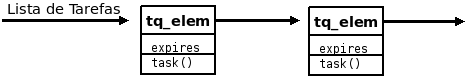
\includegraphics[scale=.8]{figs/task}
	\caption{Fila de tarefas agendadas do MIPL}
	\label{f_mipl_tasks}
\end{figure}

A \textit{thread runner}, fica percorrendo a fila de tarefas(ver figura
\ref{f_mipl_tasks}) e quando o tempo da tarefa expira, executa uma fun��o
associada, previamente registrada.

\subsubsection{\textit{icmp6\_listen}}
O MIPL cria uma \textit{thread} para escutar mensagens ICMPv6 e para isso cria
um soquete bruto. Por�m, h� muitas mensagens ICMPv6, por isso, para reduzir o
n�mero de pacotes passados do \textit{kernel} para a aplica��o, � fornecido um
filtro especifico pela aplica��o. Na tabela \ref{t_mipl_icmp} � poss�vel
observar as mensagens ICMPv6 que ser�o tratadas pelo MIPL.

\begin{table}[!htpb]
\centering
\begin{small}
  \setlength{\tabcolsep}{3pt}
\begin{tabular}{|c|c|c|c|}\hline
\raisebox{1.5ex}{Fun��o mip6d} & \raisebox{1.5ex}{Mensagem Filtrada} &
\raisebox{1.5ex}{Fun��o}\\ \hline
N� M�vel & ND\_ROUTER\_ADVERT & An�ncio de roteadores  \\ 
	 & ND\_NEIGHBOR\_ADVERT & An�ncio de vizinhan�a \\ 
	 & MIP\_HA\_DISCOVERY\_REPLY & Resposta de descoberta de agente
domiciliar \\
	 & ICMP6\_PARAM\_PROB & askdfj;al \\
	 & ICMP6\_DST\_UNREACH & Destino inalcan��vel \\ \hline
Agente Domiciliar & MIP\_PREFIX\_SOLICIT & Solicita��o de prefixo \\
		  & MIP\_HA\_DISCOVERY\_REQUEST & Descoberta de agente
domiciliar \\
		  & ND\_ROUTER\_ADVERT & An�ncio de roteadores \\
		  & ICMP6\_DST\_UNREACH & Destino inalcan��vel; \\ \hline
\end{tabular} 
\end{small}
\caption{Filtros para os pacotes ICMPv6 feitos pelo MIPL}
\label{t_mipl_icmp}
\end{table} 

Durante a execu��o do \textit{daemon} � feita a instala��o de manipuladores, que
tratam as mensagens, em uma lista global. Ao receber uma das mensagens ICMPv6
filtradas, a \textit{thread} percorre a lista de manipuladores e chama a fun��o
para tratar a mensagem.

\begin{figure}[!htpb]
	\centering
	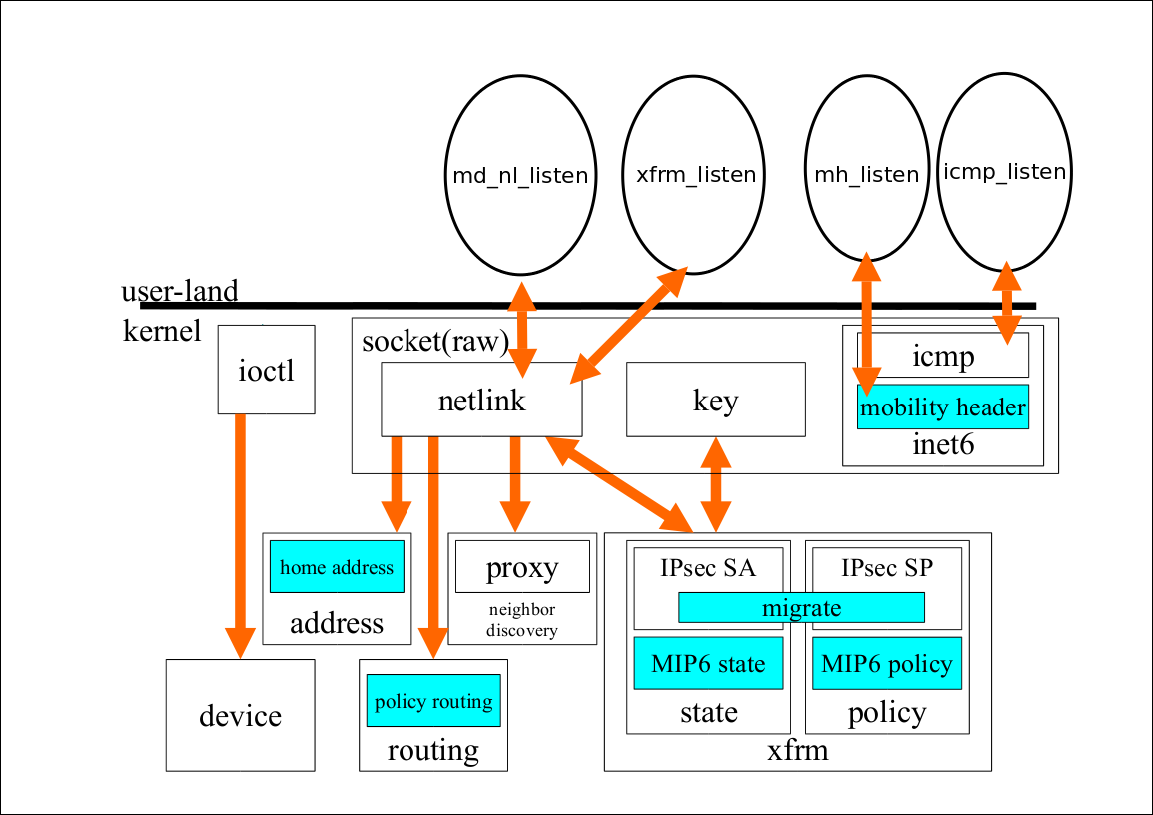
\includegraphics[scale=.27]{figs/mipl_kernel_block}
	\caption{Interfaces utilizadas pelo MIPL para fazer a comunica��o com o
kernel\cite{CitarFigura}}
	\label{f_mipl_kernel_blocks}
\end{figure}

\subsubsection{\textit{mh\_listen}}
\textit{Thread} criada para escutar a chegada de pacotes IPv6 com cabe�alho de
mobilidade. O seu funcionamento � semelhante a \textit{thread icmp6\_listen}: ao
receber uma mensagem com o cabe�alho de mobilidade chama um manipulador,
previamente instalado em uma lista global, para tratar a mensagem.

\subsubsection{\textit{xfrm\_listen}}
O \textit{daemon} cria a \textit{thread xfrm\_listen} que escuta mensagens
\textit{netlink} do \textit{framework} XFRM. Um manipulador � instalado para
tratar essas mensagens. As mensagens s�o: XFRM\_MSG\_ACQUIRE e
XFRM\_MSG\_REPORT.

\subsubsection{\textit{md\_nl\_listen}}
O \textit{mip6d} cria uma \textit{thread} para tratar mensagens \textit{netlink}
do tipo NETLINK\_ROUTE enviadas pelo \textit{kernel}. Esta \textit{thread} �
executada somente no n� m�vel.

A \textit{thread} ao receber uma mensagem \textit{netlink}, chama o manipulador
instalado para trat�-la. As mensagens tratadas pelo manipulador s�o as que
informam:
\begin{itemize}
 \item a interface ou liga��o: ligado ou desligado;
 \item as mudan�as no estado da alcan�abilidade do roteador padr�o;
 \item os \textit{Care-of-address} novos ou removidos.
\end{itemize}

\subsubsection{\textit{vt\_server\_recv}}
� possivel habilitar em tempo de compila��o um terminal virtual. O terminal
virtual permite que os usu�rios se conectem ao \textit{daemon}, via protocolo
\textit{telnet}, para obter informa��es sobre o MIPv6, por exemplo:
\begin{itemize}
 \item O tempo de vida do prefixo do agente domiciliar;
 \item O estado do \textit{Binding cache};
 \item A Lista de \textit{Bindig Updates}.
\end{itemize}

A \textit{thread} \textit{vt\_server\_recv} � criada para responder as conex�es
para o terminal virtual, que � executado na porta 7777.

\subsubsection{\textit{sigh}}
O \textit{mip6d} implementa uma \textit{thread} que � respons�vel por fazer o
tratamento de alguns sinais do sistema. Os sinais que passam a ser tratados pela
aplica��o s�o:
\begin{description}
 \item[SIGHUP:] Significa o reinicio do programa, o \textit{daemon} ao receber
esse sinal executa a fun��o \textit{reinit};
\item[SIGINT:] Causa a interrup��o do programa, em termos pr�ticos � o sinal
recebido quando se pressiona as teclas \textit{Control+C}. Neste caso ao receber
este sinal o \textit{daemon} chama a fun��o \textit{terminate};
\item[SIGTERM:] Solicita��o de t�rmino do programa, neste caso o \textit{daemon}
tamb�m chama a fun��o \textit{terminate}.
 \end{description}

� de extrema import�ncia o tratamento destes sinais pelo \textit{daemon}, pois
ao finalizar o programa � preciso deletar eventuais endere�os IP's, t�neis,
tabelas de roteamento.

\subsection{Detec��o de Movimento}
O algoritmo de detec��o de movimento do MIPL � inteiramente baseado na escuta
das mensagens de an�ncio de roteadores. O n� m�vel est� constantemente escutando
as mensagens de RA, sendo que o n� percebe o movimento quando:
\begin{itemize}
 \item o seu roteador padr�o torne-se inalcan��vel; para tanto, o n� m�vel de
tempos em tempos, verifica o roteador com um \textit{Neighbor Solicitation};
 \item passa a receber mensagens de outro roteador e para de escutar
mensagens do anterior.
\end{itemize}

Embora o MIPL seja uma extens�o da pilha IPv6 padr�o do \textit{Linux},
apresenta algumas caracter�sticas sobre administra��o de roteadores:
\begin{enumerate}
 \item O MIPL possui a sua pr�pria lista de roteadores. Esta lista cont�m o 
atual roteador de acesso, bem como roteadores que n�o s�o atualmente
utilizados, mas com tempo de vida n�o expirados;
 \item o MIPL for�a atualiza��es na tabela de roteamento ap�s receber um an�ncio
de novo roteador, e apaga todas as informa��es de roteamento que n�o s�o do
prefixo atual.
\end{enumerate}
Devido a estas duas caracter�sticas, o MIPL sempe escolhe um novo roteador. Este
m�todo de sele��o agressiva de roteadores traz uma melhora na detec��o de 
movimento, ou seja, no tempo de \textit{handover}.

\section{Altera��es no MIPL para obter o HMIPv6}
A primeira implementa��o necess�ria foi dar suporte ao MIPL a leitura das
mensagens RA divulgadas pelos MAP's, pois s�o elas que permitem a cria��o do
endere�o RCoA. No manipulador de mensagens RA foi adicionado o suporte para
a leitura da op��o de MAP na mensagem RA. Foi criada uma estrutura de dados
para o MAP e fun��es para manipula��o desta estrutura. Na estrutura de dados do
roteador foi adicionado uma lista de MAP's. A estrutura � mostrada a seguir.

\begin{lstlisting}
struct map_list_entry
{
    struct list_head list;
    struct timespec timestamp;
    struct tq_elem tqe;
    struct nd_opt_map map;
    struct in6_addr rcoa;
    int used;
};
\end{lstlisting}
A estrutura cont�m:
\begin{itemize}
 \item os campos da op��o de MAP da mensagem RA;
 \item tempo de vida do roteador que entregou a mensagem;
 \item endere�o RCoA criado a partir do endere�o do MAP;
 \item estrutura de dados que permite criar tarefas para serem agendadas;
\end{itemize}

No processamento da mensagem RA foram adicionados novos eventos de
movimento:\textbf{ME\_MAP\_NEW}, \textbf{ME\_MAP\_UPDATE} e
\textbf{ME\_MAP\_EXPIRED} Estes eventos tem a fun��o de colher os
dados que ser�o utilizados no momento do registro e  manter os dados para o
funcionamento do protocolo.

Foi criada tamb�m uma estrutura de dados para o RCoA tendo sido adicionada na
estrutura do agente domiciliar. As informa��es contidas na estrutura ser�o
utilizadas no momento da forma��o das mensagens de BU e no controle do registro.

\begin{lstlisting}
struct rcoa_addr_info {
    struct mn_addr rcoa; /* Home address for MAP */
    uint8_t mlen;
    uint8_t map_reg_status;
    struct in6_addr map_prefix;
    struct in6_addr map_addr;
    int pend_ba;
    int site;
    int if_tunnel;
};
\end{lstlisting}

Outas implementa��es foram realizadas no n� m�vel, quais sejam:
\begin {itemize}
 \item  foi acrescentado ao mecanismo de registro, um suporte ao envio do BU
para o MAP;
\item altera��o da mensagem de BU para o agente domiciliar;
\item cria��o do t�nel, com o MAP;
\item e modifica��o do t�nel com o agente domiciliar.
\end {itemize}

Algo interessante de salientar � que toda a parte de tomada de decis�o sobre o
movimento se manteve e as altera��es atuam somente na forma do registro com
os agentes.

\subsection{Detalhes do funcionamento}
A seguir, uma descri��o das implementa��es efetuadas no MIPL em um movimento
para um novo dom�nio:
\begin{enumerate}
 \item Ao receber uma mensagem RA de um novo roteador de acesso:
\begin{itemize}
 \item as op��es de MAP s�o lidas;
 \item uma lista de MAP's � criada na estrutura do roteador.
\end{itemize}
 \item Um novo MAP dispara um evento de movimento do tipo \textbf{ME\_MAP\_NEW}
que:
\begin{itemize}
 \item faz escolha de um MAP na lista de roteadores, baseado na dist�ncia em
saltos do MAP;
 \item cria um t�nel para o MAP;
 \item adiciona o RCoA na interface do t�nel;
 \item define o RCoA na estrutura do agente domiciliar, utilizado no envio do
BU.
\end{itemize}
 \item o movimento � detectado, usando o c�digo normal do MIPL. O registro
deve ser, ent�o, realizado com os agentes:
\begin{itemize}
 \item enviado BU para o MAP com os campos:
\begin{itemize}
 \item Origem = RCoA
 \item Destino = endere�o MAP
 \item Care-of-Adress = LCoA
\end{itemize}
 \item enviado BU para agente domiciliar com os campos:
 \begin{itemize}
  \item Origem = endere�o domiciliar
  \item Destino = endere�o agente domiciliar
  \item Care-of-Adress = RCoA
 \end{itemize}
\end{itemize}
 \item Ap�s o envio dos BU's, os t�neis devem ser modificados:
 \begin{itemize}
  \item T�nel entre n� m�vel e MAP: o ponto final � a interface de rede.
  \item T�nel entre n� m�vel e agente domiciliar: o ponto final � o t�nel entre
n� m�vel e MAP.
 \end{itemize}
 \item Periodicamente, com a chegada dos RA's, o evento de movimento
\textbf{ME\_MAP\_UDATE} � disparado e o tempo de vida do RCoA � atualizado.
\end{enumerate}

\subsection{Problemas conhecidos}
Considerando o car�ter experimental do trabalho, a disponibilidade de tempo
para a sua execu��o e a alta
complexidade do c�digo do MIPL, pode-se dizer que muito trabalho deve ainda ser
realizado para a obten��o de uma vers�o completa do HMIPv6. No que se refere a
implementa��o efetuada, alguns problemas podem, em particular, ser apontados:
\begin{itemize}
 \item aus�ncia de suporte a otimiza��o de rotas;
 \item aus�ncia de suporte a seguran�a (IPSec);
 \item aus�ncia de suporte ao HMIPv6 em arquivo de configura��o, somente em
tempo de compila��o;
 \item sem tarefas para deletar MAP's expirados;
 \item problema ao receber BA provindo do MAP, o que ocasiona problemas em
mobilidade em um mesmo dom�nio;
 \item problemas no retorno para rede domiciliar.
\end{itemize}

% ----------------------------------------------------------------------- %
% Arquivo: cenarios.tex
% ----------------------------------------------------------------------- %

\chapter{Cen�rios de Testes}

\section{Introdu��o}
Ap�s os estudos bibliogr�ficos sobre o protocolo MIPv6 e a prepara��o da Plataforma
 de Testes para Mobilidade, iniciou-se a etapa de defini��o e implementa��o de cen�rios
 com fins de analisar as funcionalidade dos protocolos.

Para analisar alguns mecanismos do protocolo e testar seus modos de opera��o, dois 
 cen�rios base foram definidos. Nesses dois cen�rios foi realizada tr�s simula��es.
 A primeira simula��o ocorre no cen�rio 1, descrito na figura \ref{f_cenario1}, onde
 � testado o modo de opera��o por tunelamento bi-direcional do MIPv6. A segunda simula��o
 tambem ocorre no cen�rio 1, sendo testado o modo de opera��o por otimiza��o de roteamento
 A terceira simula��o � no cen�rio 2, descrito na figura\ref{f_cenario2}, tendo como
 objetivo o funcionamento do HMIPv6.

%O computador que ser� utilizado para a realiza��o dos cen�rios de teste possui as seguintes 
% caracteristicas: \textit{Atlhon XP 2600}, 512MB de mem�ria e rodando \textit{Gnu/Linux 
% Slackware} 12.0, kernel linux-2.6.21.5.

Os arquivos para a configura��o dos cen�rios usados no Guml4Mip est�o dispon�veis no
 diret�rio da documenta��o do projeto.

%Para auxiliar na gera��o de \textit{logs}, que tendem a enriquecer an�lise dos cen�rios, foram utilizadas as ferramentas
%\textit{tcpdump}, \textit{ping6} e \textit{gen}.

\section{Fundamentos para a An�lise dos Cen�rios}
  Na an�lise dos cen�rios estudados vamos localizar os seguintes aspectos:
\begin{itemize}
  \item a sequ�ncia e a natureza das mensagens trocadas entre os v�rios n�s. Neste
 aspecto, utilizaremos as sa�das geradas pelos programas \textit{tcpdump};
  \item as tabelas de roteamento e regras de roteamento analisadas em situa��es chave,
 por exemplo, antes e depois da mobilidade;
  \item aspectos de desempenho e perdas de pacotes. Sabemos das limita��es desta an�lise 
 em um ambiente virtual, mas esperamos obter dados relativos. Tamb�m confrontaremos os dados
 obtidos com os resultados esperados segundo uma abordagem anal�tica.
  \item A cria��o e a manipula��o dos tuneis entre o agente domiciliar e o n� m�vel antes
 e depois do movimento.
\end{itemize}

\subsection{Tempo de lat�ncia do \textit{Handover}}
O processo de \textit{handover} acontece quando o n� m�vel muda seu ponto de conex�o 
 de uma sub-rede para outra. O tempo de lat�ncia envolvido neste processo \cite{xavier}
 pode ser dividida em quatro fases:

\begin{enumerate}
 \item \textbf{Detec��o de Movimento (\textit{TD})}: Em um cen�rio real representaria
 o tempo do \textit{handover} na camada de enlace at� o primeiro \textit{Router Advertisement}.
 Como neste ambiente de testes n�o conseguimos simular a camada enlace n�o se pode precisar
 com a exatid�o a lat�ncia envolvida no processo. Por�m, para fins de estudo consideraremos
 para nosso cen�rio o tempo entre o �tlimo pacote do \textit{gen} recebido na rede
 domiciliar e o primeiro \textit{Router Advertisement} na rede visitada.

\begin{equation}
 TD = t1 - t0
\label{eq.td}
\end{equation}

\item \textbf{Configura��o do \textit{Care-of-address} (\textit{TA})}: Tempo que entre 
 o primeiro \textit{Router Advertisement} e o envio do \textit{Binding Update}.

\begin{equation}
 TA = t2 -t1
 \label{eq.ta}
\end{equation}

\item \textbf{Registro com agente domiciliar (\textit{TR})}: Intervalo de tempo entre
 o envio do \textit{Binding Update} ao agente domiciliar e o recebimento do
 \textit{Binding Acknowledgement}.

\begin{equation}
 TR = t3 - t2
 \label{eq.tr}
\end{equation}

\item \textbf{Otimiza��o de Roteamento (\textit{TO})}: Intervalo de tempo entre o envio
 das mensagens do \textit{Return Routability Procedure} e o recebimento do
 \textit{Binding Acknowledgement} do n� correspondente.

\begin{equation}
 TO = t4 - t3
 \label{eq.to}
\end{equation}

\end{enumerate}

Obviamente podemos calcular o tempo de lat�ncia do handover com a seguinte f�rmula:

\begin{equation}
 TH = TD + TA + TR + TO
 \label{eq.th}
\end{equation}

\section{Cen�rio 1}
\label{s_cenario1}
O primeiro cen�rio de teste � formado por tr�s redes interligadas entre si e cinco n�s. A sua topologia pode ser observada na figura \ref{f_cenario1}, onde o numero nos bal�es cinza representam a vlan no \textit{uml-switch}. Os endere�os atribu�dos as interfaces dos n�s, durante a realiza��o do cen�rio, bem como seus endere�os de hardware est�o dispon�veis na tabela \ref{t_addr1}.

\begin{figure}[!htpb]
	\centering
	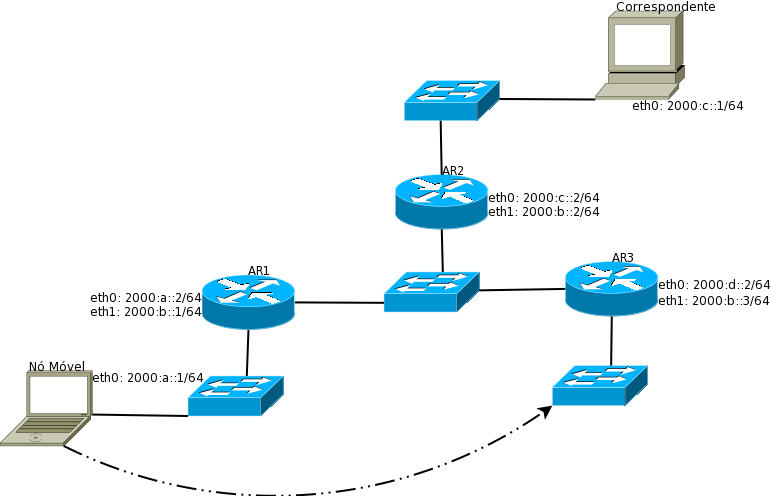
\includegraphics[scale=.4]{figs/cenario1}
	\caption{Topologia do Cen�rio 1}
	\label{f_cenario1}
\end{figure}


Na rede com prefixo 2000:a::/64 est� o n� correspondente com quem o n� m�vel est� se comunicando. Na rede com o prefixo
 2000:c::/64 est� presente um roteador (HA) que oferece o servi�o de agente domiciliar ao n� m�vel. A rede com prefixo
 2000:d::/64 � a rede que o n� m�vel deve visitar.

\begin{table}[!htpb]
\centering
\begin{small}
  \setlength{\tabcolsep}{3pt}
\begin{tabular}{|c|c|c|c|c|}\hline
\raisebox{1.5ex}{N�} & \raisebox{1.5ex}{Interface} & \raisebox{1.5ex}{MAC} & \raisebox{1.5ex}{Endere�o} & \raisebox{1.5ex}{Tipo}\\ \hline
% MN
& & & 2000:a::1 & Domiciliar (Global) \\ 
MN & eth0 & 92:09:4F:D5:EF:EA & 2000:a::9009:4fff:fed5:efea & Auto-configurado \\
& & & 2000:d::9009:4fff:fed5:efea & Care-of-address \\
& & & fe80::9009:4fff:fed5:efea & Local \\ \hline
% CN
CN & eth0 & D6:7F:B0:C3:C9:0C & 2000:c::1 & Global \\ 
& & & fe80::d47f:b0ff:fec3:c90 & Local \\ \hline
% AR1
& eth0 & AE:4D:A8:10:EB:1D & 2000:a::2 & Global \\ 
AR1 & & & fe80::ac4d:a8ff:fe10:eb1d & Local \\
& eth1 & 1E:2D:C8:43:E6:C7 & 2000:b::1 & Global \\ 
& & & fe80::1c2d:c8ff:fe43:e6c7 & Local \\ \hline
%AR2
& eth0 & 36:A7:3F:06:58:8D & 2000:c::2 & Global \\ 
AR2 & & & fe80::34a7:3fff:fe06:588d & Local \\ 
& eth1 & 4A:19:FD:12:48:34 & 2000:b::2 & Global \\
& & & fe80::4819:fdff:fe12:4834 & Local \\ \hline
%AR3
& eth0 & B2:4C:E9:EC:6C:42 & 2000:d::2 & Global \\ 
AR3 & & & fe80::b04c:e9ff:feec:6c42 & Local \\ 
& eth1 & 2A:E2:57:C7:4F:E4 & 2000:b::3 & Global \\
& & & fe80::28e2:57ff:fec7:4fe4 & Local \\ \hline
\end{tabular} 
\end{small}
\caption{Endere�os do Cen�rio 1}
\label{t_addr1}
\end{table} 


\subsection{Simula��o 1}

A simula��o 1 ter� a seguinte sequ�ncia. No in�cio o n� correspondente come�a a enviar mensagens ICMP por meio do \textit{ping6} para o n� m�vel.

\begin{verbatim}
cn# ping6 2001:a::2
\end{verbatim}

O n� m�vel realiza o monitoramento de todo o funcionamento do MIPv6 durante o processo de \textit{handover} utilizando o \textit{tcpdump} em o modo \textit{verbose} (-vvv) e para mostrar o conte�do do pacote em hexadecimal (-X).

\begin{verbatim}
mn# tcpdump -vvvX
\end{verbatim}

\subsubsection{Troca de Mesagens}
Os dados obtidos na sa�da do comando \textit{tcpdump} foram compilados em forma de uma tabela para facilitar a visualiza��o dos mesmos e podem ser observados na tabela \ref{t_resul_1}.
Analisando os dados recolhidos conseguimos observar exato momento que ocorreu a mobilidade para a outra rede. No instante entre o ICMP reply X e o RA recebido � o perio que o n� m�vel realiza o movimento.

\subsubsection{Tabelas de Roteamento}
Podemos constatar mudan�as nas tabelas de roteamento do n� m�vel e do agente domiciliar depois da mobilidade nas respecitivas figuras \ref{t_rot_mn1} e \ref{t_rot_ha1}, ap�s receber o \textit{Binding Update} e o agente domiciliar criar o t�nel com o n� m�vel, � adicionada a seguinte rota a sua tabela de roteamento, que todos os pacotes com destino ao endere�o domiciliar devem ser encaminhados para o t�nel. E no n� m�vel os pacotes com destino ao n� correspondente e ao agente domiciliar s�o encaminhados pelo t�nel, caracterizando o tunelamento bidirecional.

\subsubsection{Regras de Roteamento}

\subsubsection{Tuneis}


\begin{table}[!htpb]
\centering
\begin{small}
  \setlength{\tabcolsep}{3pt}
\begin{tabular}{|c|c|c|c|}\hline
\raisebox{1.5ex}{Destino} & \raisebox{1.5ex}{Via} & \raisebox{1.5ex}{Proximo salto} & \raisebox{1.5ex}{Considera��es}\\ \hline
default & eth0 & fe80::ac4d:a8ff:fe10:eb1d & Na rede domiciliar \\ \hline
default & eth0 & fe80::b04c:e9ff:feec:6c42 & \\ 
2000:a::2 & ip6tnl1 & 2000:a::2 & Na rede visitada \\ 
2000:c::1 & ip6tnl1 & 2000:c::1 & \\ \hline
\end{tabular} 
\end{small}
\caption{Tabela de roteamento do n� m�vel}
\label{t_rot_mn1}
\end{table} 

\begin{table}[!htpb]
\centering
\begin{small}
  \setlength{\tabcolsep}{3pt}
\begin{tabular}{|c|c|c|c|}\hline
\raisebox{1.5ex}{Destino} & \raisebox{1.5ex}{Via} & \raisebox{1.5ex}{Proximo salto} & \raisebox{1.5ex}{Considera��es} \\ \hline
2000:c::/64 & eth1 & 2000:b::2 &  Antes da mobilidade do n� m�vel \\ 
2000:d::/64 & eth1 & 2000:b::3 &   \\ \hline
2000:c::/64 & eth1 & 2000:b::2 & \\
2000:d::/64 & eth1 & 2000:b::3 & Ap�s a mobilidade do n� m�vel \\
2000:a::1 & ip6tnl1 & 2000:a::1 & \\ \hline
\end{tabular} 
\end{small}
\caption{Tabela de roteamento do agente domiciliar}
\label{t_rot_ha1}
\end{table} 

\begin{table}[!htpb]
\centering

\begin{small}
  \setlength{\tabcolsep}{3pt}
\begin{tabular}{|c|c|c|c|}\hline
\raisebox{1.5ex}{Tempo (s)} & \raisebox{1.5ex}{Origem} & \raisebox{1.5ex}{Destino} & \raisebox{1.5ex}{Conte�do}\\ \hline
21:59.952226 & fe80::ac4d:a8ff:fe10:eb1d & ff02::1 & RA, Flags [Home Agent]\\
22:00.525313 & fe80::ac4d:a8ff:fe10:eb1d & 2000:a::1 & NS, who 2000:a::1\\
22:00.525398 & 2000:a::1 & fe80::ac4d:a8ff:fe10:eb1d & Neighbor Advertisement\\
22:00.656486 & 2000:c::1 & 2000:a::1 & Gen seq\#=5\\ 
22:01.664448 & 2000:c::1 & 2000:a::1 & Gen seq\#=6\\ \hline
\textbf{22:03.467587} & \textbf{fe80::b04c:e9ff:feec:6c42} & \textbf{ff02::1} & \textbf{Router Advertisement}\\
22:03.482118 & :: & ff02::16 & HBH, multicast listener\\
22:03.799224 & :: & ff02::1:ffd5:efea & NS, who fe80::9009:4fff:fed5:efea\\
22:04.285049 & :: & ff02::1:ffd5:efea & NS, who 2000:d::9009:4fff:fed5:efea\\ 
\textbf{22:05.288026} & \textbf{2000:d::9009:4fff:fed5:efea} & \textbf{2000:a::2} & \textbf{BU seq\#=26356 AH}\\
22:05.304531 & fe80::9009:4fff:fed5:efea & ff02::16 & HBH, multicast listener\\
22:06.305532 & fe80::b04c:e9ff:feec:6c42 & ff02::1:ffd5:efea & NS, who 2000:d::9009:4fff:fed5:efea\\
22:06.305650 & 2000:d::9009:4fff:fed5:efea & fe80::b04c:e9ff:feec:6c42 & Neighbor Advertisement\\
\textbf{22:06.305972} & \textbf{2000:a::2} & \textbf{2000:d::9009:4fff:fed5:efea} & \textbf{BA seq\#=26356 lifetime=262140}\\
22:06.316950 & fe80::b04c:e9ff:feec:6c42 & ff02::1 & Router Advertisement\\
22:06.512529 & fe80::9009:4fff:fed5:efea & fe80::ac4d:a8ff:fe10:eb1d & NS, who fe80::ac4d:a8ff:fe10:eb1d\\
22:06.700567 & 2000:a::2 & 2000:d::9009:4fff:fed5:efea & 2000:c::1 > 2000:a::1 (Gen seq\#=11)\\
22:07.510304 & fe80::9009:4fff:fed5:efea & fe80::ac4d:a8ff:fe10:eb1d & NS, who fe80::ac4d:a8ff:fe10:eb1d\\
22:07.705972 & 2000:a::2 & 2000:d::9009:4fff:fed5:efea & 2000:c::1 > 2000:a::1 (Gen seq\#=12)\\
22:08.338339 & fe80::b04c:e9ff:feec:6c42 & ff02::1 & Router Advertisement\\
. & . & . & .\\
. & . & . & .\\
. & . & . & .\\
22:18.785859 & 2000:a::2 & 2000:d::9009:4fff:fed5:efea & 2000:c::1 > 2000:a::1 (Gen seq\#=23)\\ \hline
\textbf{22:19.815983} & \textbf{fe80::ac4d:a8ff:fe10:eb1d} & \textbf{ff02::1} & \textbf{RA, Flags [Home Agent]}\\
22:19.839337 & :: & ff02::16 & HBH, multicast listener\\
22:19.877057 & :: & ff02::16 & HBH, multicast listener\\
22:20.170279 & :: & ff02::1:ffd5:efea & NS, who 2000:a::9009:4fff:fed5:efea\\
22:20.585230 & :: & ff02::1:ffd5:efea & NS, who fe80::9009:4fff:fed5:efea\\
22:20.879643 & :: & ff02::16 & HBH, multicast listener\\
22:21.585309 & :: & ff02::1:ff00:1 & NS, who 2000:a::1\\
22:21.606725 & fe80::9009:4fff:fed5:efea & ff02::16 & HBH, multicast listener\\
22:21.767709 & fe80::ac4d:a8ff:fe10:eb1d & ff02::1 & Neighbor Advertisement\\
\textbf{22:21.772629} & \textbf{2000:a::1} & \textbf{2000:a::2} & \textbf{BU seq\#=26357}\\
22:21.785931 & fe80::9009:4fff:fed5:efea & ff02::16 & HBH, multicast listener \\
22:21.792882 & fe80::ac4d:a8ff:fe10:eb1d & ff02::16 & HBH, multicast listener \\
22:21.812524 & fe80::ac4d:a8ff:fe10:eb1d & ff02::1:ff00:1 & NS, who 2000:a::1 \\
22:21.812620 & 2000:a::1 & fe80::ac4d:a8ff:fe10:eb1d & Neighbor Advertisement \\
22:21.812932 & 2000:c::1 & 2000:a::1 & Gen seq\#=27 \\
\textbf{22:21.874997} & \textbf{2000:a::2} & \textbf{2000:a::1} & \textbf{BA seq\#=26357 lifetime=0} \\
22:21.904397 & 2000:a::1 & ff02::1 & Neighbor Advertisement \\
22:22.569757 & fe80::ac4d:a8ff:fe10:eb1d & ff02::1 & RA, Flags [Home Agent] \\
22:22.814652 & 2000:c::1 & 2000:a::1 & Gen seq\#=28 \\ \hline
\end{tabular} 
\end{small}
\caption{Mensagens do Cen�rio 1 com Tunelamento Bidirecional}
\label{t_resul_1}
\end{table} 


\begin{table}[!htpb]
\centering
\begin{small}
  \setlength{\tabcolsep}{3pt}
\begin{tabular}{|c|c|c|c|}\hline
\raisebox{1.5ex}{Tempo (s)} & \raisebox{1.5ex}{Origem} & \raisebox{1.5ex}{Destino} & \raisebox{1.5ex}{Conte�do}\\ \hline
50:21.991721 & 2000:a::1 & 2000:c::1 & ICMP6, echo reply \\ \hline
\textbf{50:24.231519} & \textbf{fe80::b04c:e9ff:feec:6c42} & \textbf{ff02::1} & \textbf{Router Advertisement}\\
50:24.247992 & :: & ff02::16 & HBH, multicast listener\\
50:24.545598 & :: & ff02::1:ffd5:efea & NS, who 2000:d::9009:4fff:fed5:efea\\ 
50:24.879467 & :: & ff02::1:ffd5:efea & NS, who fe80::9009:4fff:fed5:efea\\
50:25.548165 & fe80::b04c:e9ff:feec:6c42 & ff02::1 & Router Advertisement\\
\textbf{50:25.557223} & \textbf{2000:d::9009:4fff:fed5:efea} & \textbf{2000:a::2} & \textbf{BU seq\#=47808 AH}\\
50:25.576407 & :: & ff02::16 & HBH, multicast listener\\
50:26.581135 & fe80::b04c:e9ff:feec:6c42 & ff02::1:ffd5:efea & NS, who 2000:d::9009:4fff:fed5:efea\\
50:26.581276 & 2000:d::9009:4fff:fed5:efea & fe80::b04c:e9ff:feec:6c42 & Neighbor Advertisement\\
\textbf{50:26.581588} & \textbf{2000:a::2} & \textbf{2000:d::9009:4fff:fed5:efea} & \textbf{BA seq\#=47808 lifetime=262140}\\ \hline
50:26.987535 & fe80::9009:4fff:fed5:efea & fe80::ac4d:a8ff:fe10:eb1d & NS, who fe80::ac4d:a8ff:fe10:eb1d\\
50:27.009344 & 2000:a::2 & 2000:d::9009:4fff:fed5:efea & 2000:c::1 > 2000:a::1, (icmp6)\\
50:27.009538 & 2000:d::9009:4fff:fed5:efea & 2000:a::2 & 2000:a::1 > 2000:c::1,(icmp6)\\
\textbf{50:27.013543} & \textbf{2000:d::9009:4fff:fed5:efea} & \textbf{2000:a::2} & \textbf{2000:a::1 > 2000:c::1,(HoTI)}\\
\textbf{50:27.015165} & \textbf{2000:d::9009:4fff:fed5:efe} & \textbf{2000:c::1} & \textbf{CoTI Care-of Init}\\
\textbf{50:27.019919} & \textbf{2000:a::2} & \textbf{2000:d::9009:4fff:fed5:efea} & \textbf{2000:c::1 > 2000:a::1, (HoT)}\\
\textbf{50:27.029192} & \textbf{2000:c::1} & \textbf{2000:d::9009:4fff:fed5:efea} & \textbf{CoT}\\
\textbf{50:27.031650} & \textbf{2000:d::9009:4fff:fed5:efea} & \textbf{2000:c::1} & \textbf{BU seq\#=1077 A}\\
\textbf{50:27.037401} & \textbf{2000:c::1} & \textbf{2000:d::9009:4fff:fed5:efea} & \textbf{BA seq\#=1077 lifetime=420}\\
50:27.365152 & fe80::b04c:e9ff:feec:6c42 & ff02::1 & Router Advertisement\\
50:27.982719 & fe80::9009:4fff:fed5:efea & fe80::ac4d:a8ff:fe10:eb1d & Neighbor Solicitation\\
50:28.014358 & 2000:c::1 & 2000:d::9009:4fff:fed5:efea & ICMP6, echo request\\
50:28.014494 & 2000:d::9009:4fff:fed5:efea & 2000:c::1 & ICMP6, echo reply \\ \hline
\end{tabular} 
\end{small}
\caption{Mensagens do Cen�rio 1 com Otimiza��o de Roteamento}
\label{t_mes_ro}
\end{table} 

Na tabela \ref{t_handover}, encontram-se os tempos das fases do processo de \textit{handover} referentes ao cen�rio estudado.

\begin{table}[!htpb]
\centering
\begin{small}
  \setlength{\tabcolsep}{3pt}
\begin{tabular}{|c|c|c|}\hline
\raisebox{1.5ex}{Fase} & \raisebox{1.5ex}{Tempo (ms)} & \raisebox{1.5ex}{Media \%} \\ \hline
\textit{TD} & 2240 & 48,6 \\ \hline
\textit{TA} & 1320 & 28.63\\ \hline
\textit{TR} & 1030 & 22.34\\ \hline
\textit{TO} & 20 &  0.43\\ \hline
\textit{TH} & 4610 & 100 \\ \hline
\end{tabular} 
\end{small}
\caption{Lat�ncia no \textit{Handover} do cen�rio estudado}
\label{t_handover}
\end{table} 

Utilizando o cen�rio estudado como refer�ncia, foi realizado um teste que pretende verificar a perda na taxa de transmiss�o em um processo de \textit{handover}. Utilizando a ferramenta \textit{gen} que permite gerar tr�fegos espec�ficos e relat�rios que extraem a taxa de trasmiss�o e a perda de pacotes, e utilizando o utilit�rio \textit{GNUPLOT} somos capazes de gerar gr�ficos que avaliam esse desempenho.

Os testes realizados foram feitos utilizando tunelamento bidirecional, o tempo configurado para o intervalo entre as mensagens de \textit{Router Advertisement} foi de 30 � 70 milisegundos. Os comandos disparados nos n�s m�vel e correspondente foram os seguintes:
\begin{verbatim}
mn# gen -l -d -p udp -s 14000 -f /host/log/
cn# gen -a 2000:a::1 -d -p udp -s 14000
\end{verbatim}

O gr�fico obtido no teste, pode ser observado na figura \ref{f_banda}.

\begin{figure}[!htpb]
	\centering
	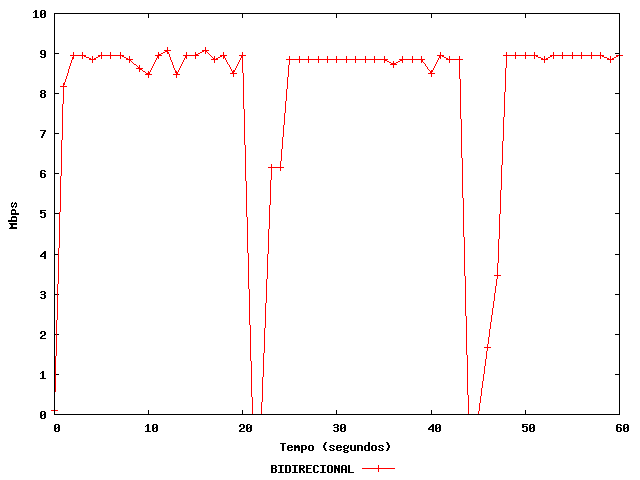
\includegraphics[scale=.6]{figs/banda}
	\caption{Taxa de transmiss�o em \textit{Handover}}
	\label{f_banda}
\end{figure}

A partir dos dados levantados com o teste podemos tirar v�rias conclus�es, entre as quais destacam-se que o \textit{Troughput} suportado pela rede gira em torno de 9 Mbps, este dado esta muito relacionado ao desempenho da m�quina hospedeiro, que cada \textit{handover} � de aproximadamente 3 segundos, h� perdas consider�veis de pacotes que prejudicariam muito comunica��es interativas como videoconfer�ncia e \textit{VoIP}, por�m, navega��o em paginas da \textit{Internet} e visualiza��o de \textit{e-mail} a instabilidade � toler�vel.

Como cen�rio estudo foi simulado todos os tempos medidos s�o estimados. Por�m, segundo algumas bibliografias estudadas que realizaram experimentos fisicamente os tempos medidos na simula��o est�o dentro do esperado.

� percept�vel que as fases que mais comprometem o \textit{handover} do nosso cen�rio s�o as da detec��o de movimento e a configura��o do \textit{care-of-address}. Algumas tentativas podem ser feitas para tentar diminuir a lat�ncia nestas duas fases.

Na tentativa de diminuir o tempo da fase de detec��o de movimento, podemos diminuir o intervalo entre as mensagens de \textit{Router Advertisement} do roteador presente na rede que ir� ser visitada pelo n� m�vel. Pois, � por meio desta mensagem que o n� m�vel detecta o movimento e desencadeia todo o processo de \textit{handover}.

No intuito de verificar se h� uma melhora no processo de handover. O cen�rio estudado foi repetido variando o intervalo entre as mensagens de \textit{Router Advertisement}. O resultado deste teste esta dispon�vel na figura \ref{f_radvd}.

\begin{figure}[!htpb]
	\centering
	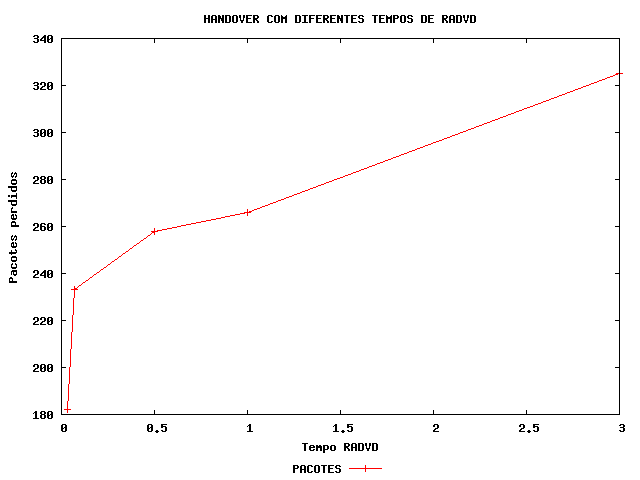
\includegraphics[scale=.6]{figs/radvd}
	\caption{Diferentes intervalos entre as mensagens \textit{Router Advertisement}}
	\label{f_radvd}
\end{figure}

Com os dados levantados, � poss�vel perceber que o intervalo entre as mensagens de \textit{Router Advertisement} esta diretamente ligado com a perda de pacotes durante o \textit{handover}. Por�m, esta n�o � uma boa pr�tica para tentar amenizar a lat�ncia do handover, pois um numero muito grande de mensagens \textit{multicasting} inundaria a rede prejudicando a perfomance principalmente em redes sem fio.

No processo de forma��o de um novo \textit{care-of-address} o DAD � necess�rio para se certificar que o endere�o formado � exclusivo. Para o teste ser bem sucedido nenhum n� vizinho deve enviar um \textit{Neighbor Advertisement}, em resposta ao teste, ou \textit{Neighbor Solicitation}, como o mesmo endere�o em quest�o, em um per�odo de \textit{1000ms} segundo a RFC 2462 \cite{rfc2462}. Este tempo de espera compromete a fase de configura��o do \textit{care-of-address}.

Existe uma vari�vel chamada \textit{dad\_transmits} no kernel do Linux que � usada para configurar o DAD em um n�. Com a inten��o de diminuir a lat�ncia na fase de configura��o do \textit{care-of-address}, n�s configuramos a vari�vel com o valor 0, isso significa que o procedimento de DAD � cancelado, e repetimos o cen�rio estudado.

\section{Resultados}
Com a realiza��o dos experimentos podemos constatar o funcionamento do protocolo e perceber continua��o da comunica��o entre os pontos comunicantes ap�s a mobilidade de forma transparente as camadas superiores a de rede, observar todas as mensagens trocadas no processo e estimar o tempo de lat�ncia com a mobilidade.
O primeiro resultado que se pode obter com a realiza��o do Cen�rio 1, foi o perfeito funcionamento do MIPv6, ocorreram algumas perdas de pacotes, mas o n� m�vel conseguiu continuar sendo alcan�ado pelo seu endere�o domiciliar mesmo n�o estando em sua rede domiciliar.

\section{Cen�rio 2}
\label{s_cenario2}


\begin{figure}[!htpb]
	\centering
	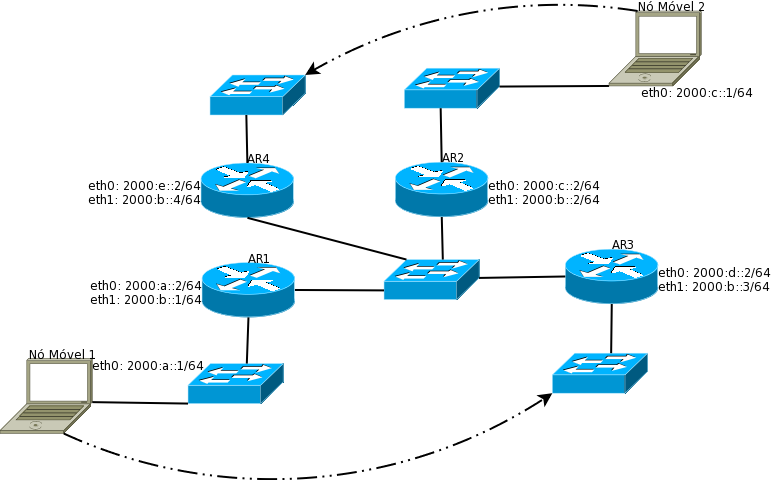
\includegraphics[scale=.37]{figs/cenario2}
	\caption{Topologia do Cen�rio 2}
 	\label{f_cenario2}
\end{figure}

% ----------------------------------------------------------------------- %
% Arquivo: conclusoes.tex
% ----------------------------------------------------------------------- %

\chapter{Conclus�es}
\label{c_conclusoes}

Este trabalho procurou mostrar como dever� ser a apresenta��o da monografia a ser submetida � Coordena��o do Curso Superior de Tecnologia em Sistemas de Telecomunica��es do Centro Federal de Educa��o Tecnol�gica de Santa Catarina para a obten��o do diploma de Tecn�logo em Sistemas de Telecomunica��es.

No cap�tulo \ref{c_introducao} foi feita uma pequena introdu��o. No cap�tulo  foram apresentados alguns coment�rios sobre figuras. E no cap�tulo  foi apresentada uma forma para inserir tabela.

Como trabalho futuro, fica a reescrita do texto deste documento de forma que ele possam indicar informa��es espec�ficas a formata��o do documento. Como o tamanho da fonte utilizada, o espa�amento da borda, o alinhamento e n�mera��o das se��es e cap�tulos, etc.
% inclus�o de ap�ndices (se houver)
\apendice
% ----------------------------------------------------------------------- %
% Arquivo: ipv6.tex
% ----------------------------------------------------------------------- %
\chapter{IPv6}
\label{c_anexo_ipv6}
Considerando o grande crescimento da \textit{Internet}, o protocolo que �
utilizado hoje, o \acf{IPv4}, � considerado incapaz de suprir a necessidade da
demanda por novos endere�os na \textit{Internet}.

A previs�o atual para a exaust�o de todos os endere�os IPv4 livres � Mar�o 2011
\cite{ipv4}, o que significa que o uso do \acf{IPv6} � inevit�vel num futuro
pr�ximo.

Com o intuito de resolver o problema de n�meros de endere�o e as principais
falhas encontradas no IPv4, foi proposto o protocolo IPv6. As principais
melhorias s�o:

\begin{itemize}
	\item  Amplia��o do Espa�o de Endere�amento de 32 bits para 128 bits;
	\item  Melhoria na estrutura (formato) do pacote IP;
	\item  Melhoria no processo de autoconfigura��o;
	\item  Inser��o de mecanismos para tratamento de mobilidade, seguran�a e
facilidades para o gerenciamento de \ac{QoS}.
\end{itemize}

\section{A estrutura de cabe�alhos}

Um datagrama IPv6 � constitu�do por um cabe�alho base de tamanho fixo de 40
bytes, seguido de zero ou mais cabe�alhos de extens�o. Na figura \ref{f_ipv6}, �
ilustrado um cabe�alho IPv6 com um cabe�alho de exten��o de mobilidade.
\begin{figure}[!htpb]
	\centering
	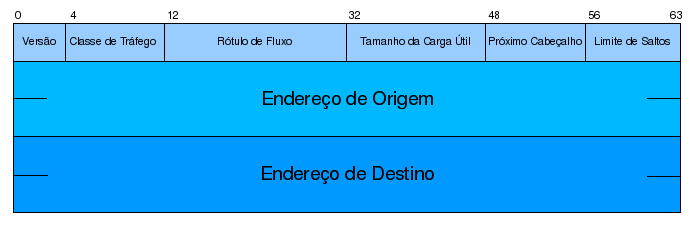
\includegraphics[scale=1]{figs/ipv6}
	\label{f_ipv6}
	\caption{Estrutura do Cabe�alho do IPv6}
\end{figure}

O fato do cabe�alho IPv6 possuir um tamanho fixo � uma vantagem, pois acelera o
processamento dos pacotes nos roteadores, uma vez que n�o h� necessidade de
calcular o tamanho de alguns campos e do cabe�alho como um todo.

A redu��o do n�meros de campos utilizados, excluindo os campos com pouca
utilidade pr�tica, tamb�m contribui para a diminui��o do tempo gasto em
processamento pelos roteadores. Entre eles, dois que merecem destaque,
\textit{checksum} e o de fragmenta��o.

A fun��o do campo de \textit{checksum} era detectar erros que afetassem ao
cabe�alho IP, n�o detectando no entanto erros no restante do pacote. Hoje os
mecanismos de dete��o de erros Ethernet e PPP s�o bastante eficientes, o que
permitiu a exclus�o do campo \textit{checksum}. Com isso os roteadores n�o
precisam recalcular o \textit{checksum} a cada salto, melhorando a sua
performace.

Quanto ao campo fragmenta��o, este foi exclu�do, pois decidiu-se que pacotes n�o
ser�o mais fragmentados por roteadores. Caso algum roteador da rota detecte que
o pacote � muito grande para o \ac{MTU} ent�o ele avisa o n� fonte com ICMPv6
\textit{Packet Too Big}, que inclui o tamanho da MTU do enlace problema.

Desta forma h� um ganho de performance no roteamento, pois � eliminada a
necessidade de um roteador fragmentar v�rios pacotes.
 
\section{O endere�amento IPv6}
O endere�amento no IPv6 passa a ser de 128 bits, incluindo o prefixo de rede e
sufixo do host. N�o existem classes de endere�os, como acontecia no IPv4.

Os endere�os IPv6 s�o representados normalmente como oito grupos de 4 d�gitos
hexadecimais. Por exemplo:
\begin{verbatim}
   3ffe:88a6:3a58:3d8a:021e:8cff:fe91:f6dd
\end{verbatim}
Se um grupo de d�gitos for zeros, eles pode ser omitido. Por exemplo: 
\begin{verbatim}
   3ffe:88a6:3a58:0000:0000:0000:0000:f6dd 
\end{verbatim}
� o mesmo endere�o IPv6 que: 
\begin{verbatim}
   3ffe:88a6:3a58::f6dd
\end{verbatim}
No IPv6 existem tr�s tipos de endere�os:
\begin{itemize}
 \item \textit{unicast} - cada endere�o identifica uma interface (dispositivo).
 \item \textit{multicast} - cada endere�o identifica m�ltiplas interfaces. �
enviada uma c�pia para cada interface. O IPv6 eliminou o \textit{broadcast} e
enriqueceu o processo de \textit{multicast};
 \item \textit{anycast} - cada endere�o pode ser atribu�do a m�ltiplas
interfaces. Um datagrama � enviado para um dos dispositivos, por exemplo, o mais
pr�ximo.
\end{itemize}

\section{ICMPv6}

O \acf{ICMPv6} \cite{rfc4443} permite enviar mensagens de erro e informa��o.

Em compara��o ao \acf{ICMPv4}, podedos citar dentro das principais mudan�as para
o ICMPv6 a incorpora��o da fun��o de converter o endere�o IP em endere�o f�sico,
fun��o que no IPv4 era feita por um protocolo a parte, o \ac{ARP} \cite{rfc826}.

As mensagens de descoberta de informa��es de vizinhan�a \acf{ND},
podem ser usadas para desempenhar a fun��o equivalente ao ARP/RARP, para
detec��o de IP duplicado \acf{DAD}, fazer an�ncio ou solita��o de roteadores e
outros.

O protocolo \ac{IGMP} que trata o multicast tamb�m foi incorporado no ICMPv6.

No \ac{MIP}, para fazer os registro de localiza��o, tamb�m � utilizado
as mensagens ICMP.

\section{Autoconfigura��o}

A autoconfigura��o � um dos pontos fortes do IPv6. Ela viza liberar o usu�rio da
tarefa de configura��o, tornando-a autom�tica e transparente.
Ela pode ser feita por \textit{stateful autoconfiguration}, onde o endere�o e
outros par�metros de configura��o s�o providos diretamente de um servidor, por
exemplo, os mecanismos \acf{DHCPv6} e \acf{PPPv6}. Ou pode ser feita por por
\textit{stateless autoconfiguration} \cite{rfc2462}, no qual o endere�o � gerado
combinando os prefixos divulgados pelos roteadores e o \ac{MAC} do n�.

% \include{sock}

% inclus�o de anexos (se houver)
\anexo
% ----------------------------------------------------------------------- %
% Arquivo: anexo.tex
% ----------------------------------------------------------------------- %

\chapter{Arquivo de Configura��o do GUML4MIP}
\label{c_anexo_guml4mip}
\lstinputlisting[language=C, label=guml_example, caption={Exempo de arquivo de
configura��o de uma m�quina UML, para o GUML4MIP}]{anexos/exemplo.conf}

\bibliographystyle{abnt-alf}
\bibliography{rfc}

\end{document}
